\chapter{刚体的三维运动}
\thispagestyle{empty}
\section{向量及其运算的矩阵表示}
\label{向量运算的矩阵表示}

\subsection{向量的描述及向量运算的矩阵表示}
对于任意一个\dy{向量}{XL}$\bm{u}$,都可以表示为某个\dy{向量基}{XLJ}
$\underline{\bm{e}} = \big[ \bm{i} \quad \bm{j} \quad \bm{k} \big]^\T $的\dy{基向量}{JXL}的线性组合,即
\begin{equation}
	\bm{u} = u_s \bm{i} + u_y \bm{j} + u_z \bm{k}
	\nomenclature{$\bm{u}$}{三维向量$\bm{u}$\nomrefpage}
	\nomenclature{$\bm{e}$}{三维向量基$\bm{e}$\nomrefpage}
\end{equation}
其中,$\bm{i}, \bm{j}, \bm{k}$分别称为向量$\bm{u}$在基向量上的3个分向量,3个标量系数$u_x,u_y,u_z$分别称为向量$\bm{u}$在3个基向量上的坐标。这3个坐标构成一个标量矩阵,称为向量$\bm{u}$在基向量$\bm{e}$上的\dy{坐标阵}{ZBZ}(或\dy{分量矩阵}{FLJZ}),记为
\begin{equation}
	\bm{u} = \big[ u_x \quad u_y \quad u_z \big]^\T	
\end{equation}

那么向量$\bm{u}$可以写成矩阵乘积的形式为
\begin{equation}
	\bm{u} = \bm{u}^\T \bm{e} = \bm{e}^\T \bm{u}
\end{equation}
由基向量的正交性,可以将$\bm{u}$的分量矩阵写为
\begin{equation}
	\bm{u} =
	\begin{bmatrix}
		\bm{u} \cdot \bm{i} \\
		\bm{u} \cdot \bm{j} \\
		\bm{u} \cdot \bm{k}
	\end{bmatrix}
	= \bm{u} \cdot \bm{e} = \bm{e} \cdot \bm{u}
\end{equation}


\subsection{向量叉乘的矩阵表示}
已知向量在三维坐标系下的表达为$\bm{u} = u_1\bm{i} +u_2\bm{j} +u_3\bm{k}, \, \bm{v} = v_1\bm{i} + v_2\bm{j} + v_3 \bm{k}$,其中,$\bm{i}, \bm{j}, \bm{k}$是单位标准正交基,且其运算满足表 \ref{向量叉乘} ,即满足右手系。
\begin{table}[!htb]
	\centering
	\setlength{\tabcolsep}{2.5em}{
		\begin{tabular}{|c|c|c|c|}
			\hline
			\rowcolor{Azure2} $\times$  & $ \bm{i} $ & $ \bm{j} $ & $ \bm{k} $ \\
			\hline
			\cellcolor{Azure2}  $\bm{i}$ & $0$ &\cellcolor{MistyRose} $\bm{k}$ & \cellcolor{DarkSlateGray2} $-\bm{j}$ \\
			\hline
			\cellcolor{Azure2}  $\bm{j}$ & \cellcolor{MistyRose} $-\bm{k}$ & $0$ & \cellcolor{LightGoldenrod1} $\bm{i}$ \\
			\hline
			\cellcolor{Azure2}  $\bm{k}$ & \cellcolor{DarkSlateGray2} $\bm{j}$ &  \cellcolor{LightGoldenrod1} $-\bm{i}$ & $0$ \\
			\hline
		\end{tabular}
	}
	\caption{单位标准正交向量的叉乘计算表(左$\times$上)}
	\label{向量叉乘}
\end{table}

那么,由向量叉乘的分配律及单位标准正交基的运算法则,
\vspace*{-0.5em}
\begin{align*}
	\bm{u} \times \bm{v} &= (u_1\bm{i} +u_2\bm{j} +u_3\bm{k}) \times (v_1\bm{i} + v_2\bm{j} + v_3 \bm{k}) \\
	&= u_1v_1( \bm{i} \times \bm{i}) + u_1v_2 (\bm{i} \times \bm{j}) + u_1v_3 (\bm{i} \times \bm{k} ) 
	+ u_2v_1 (\bm{j} \times \bm{i}) + u_2v_2 (\bm{j} \times \bm{j}) + u_2v_3 (\bm{j} \times \bm{k}) \\
	&+ u_3v_1 (\bm{k} \times \bm{i}) + u_3v_2 (\bm{k} \times \bm{j}) + u_3v_3 (\bm{k} \times \bm{k}) \\
	&= u_1v_2 \bm{k} + u_1v_3 (-\bm{j} )+ u_2v_1 (- \bm{k}) + u_2v_3 \bm{i} + u_3v_1 \bm{j} + u_3v_2 (-\bm{i}) \\
	&= (u_2v_3 - u_3v_2)\bm{i} + (u_3v_1 - u_1v_3) \bm{j} + (u_1v_2 - u_2v_1)\bm{k} =
	\begin{vmatrix}
		\bm{i} & \bm{j} & \bm{k} \\
		u_1 & u_2 & u_3 \\
		v_1& v_2 & v_3
	\end{vmatrix}
\end{align*}
将向量用矩阵表达,即
\begin{align*}
	\bm{u} \times \bm{v} &= (u_2v_3 - u_3v_2)\bm{i} + (u_3v_1 - u_1v_3) \bm{j} + (u_1v_2 - u_2v_1)\bm{k} \\
	& = 
	\big[ \bm{i} \quad \bm{j} \quad \bm{k} \big] \,
	\begin{bmatrix}
		u_2v_3 - u_3v_2 \\
		u_3v_1 - u_1v_3 \\
		u_1v_2 - u_2v_1
	\end{bmatrix} 
	=
	\big[ \bm{i} \quad \bm{j} \quad \bm{k} \big] \,
	\begin{bmatrix}
		0 & -u_3 & u_2 \\
		u_3 & 0 & -u_1 \\
		-u_2  &  u_1 & 0
	\end{bmatrix}
	\, 
	\begin{bmatrix}
		v_1 \\
		v_2 \\
		v_3 
	\end{bmatrix}
\end{align*}
所以,我们可以得到\dy{向量叉乘矩阵}{XLCCJZ}的定义

\defination{向量叉乘矩阵}
{
	已知向量$\bm{u} = u_1\bm{i} +u_2\bm{j} +u_3\bm{k}, \, \bm{v} = v_1\bm{i} + v_2\bm{j} + v_3 \bm{k}$,其在同一个坐标系下的叉乘运算可以用矩阵表达
	\begin{equation}
		\bm{u} \times \bm{v} = 	
		\big[ \bm{i} \quad \bm{j} \quad \bm{k} \big] \,
		\begin{bmatrix}
			0 & -u_3 & u_2 \\
			u_3 & 0 & -u_1 \\
			-u_2  &  u_1 & 0
		\end{bmatrix}
		\, 
		\begin{bmatrix}
			v_1 \\
			v_2 \\
			v_3 
		\end{bmatrix}
	=\bm{e}^\T \bm{u}^\times \bm{v} = \bm{v}^\T (\bm{u}^\times)^\T \bm{e}
	\end{equation}
	同时,叉乘矩阵有一个很重要的性质,从其定义很容易可以发现
	\begin{equation}
		(\bm{u}^\times )^\T = 
		\begin{bmatrix}
			0 & u_3 & -u_2 \\
			-u_3 & 0 & u_1 \\
			u_2  &  -u_1 & 0
		\end{bmatrix}
		= -
		\begin{bmatrix}
			0 & -u_3 & u_2 \\
			u_3 & 0 & -u_1 \\
			-u_2  &  u_1 & 0
		\end{bmatrix}
		= - \bm{u}^\times
	\end{equation}
    所以向量叉乘矩阵又称为\dy{反对称矩阵}{FDCJZ}。
}

进一步,我们将叉乘运算进一步写为分量形式后可以定义\dy{广义向量叉乘运算}{GYXLCCYS}如下。

\defination{广义向量叉乘运算}
{
	已知向量$\bm{u}, \bm{v}$在坐标系$S$下的分量形式为$\bm{u}^\T \bm{e}, \, \bm{e}^\T \bm{v}$,则
	\begin{equation}
		\bm{u}^\T \bm{e} \times \bm{e}^\T \bm{b} = \big[ \bm{i} \quad \bm{j} \quad \bm{k} \big] \,
		\begin{bmatrix}
			0 & -u_3 & u_2 \\
			u_3 & 0 & -u_1 \\
			-u_2  &  u_1 & 0
		\end{bmatrix}
		\, 
		\begin{bmatrix}
			v_1 \\
			v_2 \\
			v_3 
		\end{bmatrix}
		=\bm{e}^\T \bm{u}^\times \bm{v}
	\end{equation}
	定义广义向量叉乘运算为
	\begin{equation}
		\bm{u}^\T \bm{e} \times \bm{e}^\T = \bm{e}^\T \bm{u}^\times
	\end{equation}
}
\label{广义向量叉乘运算}



\subsection{叉乘矩阵的坐标变换}
\label{叉乘矩阵的坐标变换}
对于向量叉乘运算$\bm{w} = \bm{u} \times \bm{v}$,在坐标系$S_a,\, S_b$下的矩阵形式分别为
\begin{equation*}
	\bm{w}_a = \bm{u}_a^\times \bm{v}_a, \qquad \bm{w}_b = \bm{u}_b^\times \bm{v}_b
\end{equation*}
由$\bm{w}_a = \bm{C}_{ab} \bm{w}_b$,
\begin{equation*}
	\bm{C}_{ab} \bm{w}_b = \bm{a}^\times \bm{C}_{ab} \bm{v}_b \quad \Rightarrow \quad \bm{w}_b = \bm{C}_{ba} \bm{u}_a^\times \bm{C}_{ab} \bm{v}_b
\end{equation*}
通过对比前后两个式子可得

\theorem{叉乘矩阵的坐标变换}
{
	$\bm{u}$在坐标系$S_a, \, S_b$下的叉乘矩阵的坐标变换关系为
	\begin{equation}
		\bm{u}_b^\times = \left(\bm{C}_{ba} \bm{u}_a \right) = \bm{C}_{ba} \bm{u}_a^\times \bm{C}_{ab}
		= \bm{C}_{ba} \bm{u}_a^\times \bm{C}_{ba}^\T
	\end{equation}
	进一步,可以扩展得到\dy{叉乘矩阵恒等式}{CCJZHDS}
	\begin{equation}
		\left( \bm{C} \bm{u} \right)^\times = \bm{C} \bm{u}^\times \bm{C}^\T
	\end{equation}
}


\subsection{向量两边乘同一个向量运算的矩阵表示}
已知向量在三维坐标系下的表达为$\bm{u} = u_1\bm{i} +u_2\bm{j} +u_3\bm{k}, \, \bm{v} = v_1\bm{i} + v_2\bm{j} + v_3 \bm{k}$,则
\begin{align*}
	\bm{u} \cdot \bm{v} \cdot \bm{u}  &= (u_1\bm{i} +u_2\bm{j} +u_3\bm{k}) \cdot (v_1\bm{i} + v_2\bm{j} + v_3 \bm{k}) \bm{u} \\
	& = (u_1v_1 + u_2v_2 + u_3v_3) \bm{u} \\
	& =  (u_1v_1 + u_2v_2 + u_3v_3) (u_1\bm{i} +u_2\bm{j} +u_3\bm{k}) \\
	& = (u_1^2 v_1 + u_1u_2v_2 + u_1u_3 v_3) \bm{i} + (u_1u_2v_1 + u_2^2 v_2 + u_2u_3v_3)\bm{j} + (u_1u_3v_1 + u_2u_3v_2 + u_3^2v_3) \bm{k}
\end{align*}
用矩阵表达为
\begin{align*}
	\bm{u} \cdot \bm{v} \cdot \bm{u} &= (u_1^2 v_1 + u_1u_2v_2 + u_1u_3 v_3) \bm{i} + (u_1u_2v_1 + u_2^2 v_2 + u_2u_3v_3)\bm{j} + (u_1u_3v_1 + u_2u_3v_2 + u_3^2v_3) \bm{k} \\
	& =
	\big[ \bm{i} \quad \bm{j} \quad \bm{k} \big] \,
	\begin{bmatrix}
		u_1^2v_1 + u_1u_2 v_2 + u_1u_3 v_3 \\
		u_1u_2v_1 + u_2^2 v_2 + u_2u_3v_3 \\
		u_1u_3v_1 + u_2u_3v_2 + u_3^2v_3
	\end{bmatrix}\\[0.5em]
	& = 
	\big[ \bm{i} \quad \bm{j} \quad \bm{k} \big] \,
	\begin{bmatrix}
		u_1^2 & u_1u_2 & u_1u_3 \\
		u_1u_2 & u_2^2 & u_2u_3 \\
		u_1u_3 & u_2u_3 & u_3^2
	\end{bmatrix}
	\,
	\begin{bmatrix}
		v_1 \\
		v_2 \\
		v_3
	\end{bmatrix} \\[0.5em]
& = 
\big[ \bm{i} \quad \bm{j} \quad \bm{k} \big] \,
\begin{bmatrix}
	u_1 \\
	u_2 \\
	u_3
\end{bmatrix}
\,
\big[ u_1 \quad u_2 \quad u_3 \big]
\,
\begin{bmatrix}
	v_1 \\
	v_2 \\
	v_3
\end{bmatrix}
\end{align*}
所以,我们可以得到

\theorem{向量两边乘同一个向量运算的矩阵表示}
{
	已知向量$\bm{u} = u_1\bm{i} +u_2\bm{j} +u_3\bm{k}, \, \bm{v} = v_1\bm{i} + v_2\bm{j} + v_3 \bm{k}$,则
	\begin{equation}
		\bm{u} \cdot \bm{v} \cdot \bm{u} = 
		\big[ \bm{i} \quad \bm{j} \quad \bm{k} \big] \,
		\begin{bmatrix}
			u_1 \\
			u_2 \\
			u_3
		\end{bmatrix}
		\,
		\big[ u_1 \quad u_2 \quad u_3 \big]
		\,
		\begin{bmatrix}
			v_1 \\
			v_2 \\
			v_3
		\end{bmatrix}
		= \bm{e}^\T \bm{u} \bm{u}^{\text{T}} \bm{v} =\bm{v}^\T \bm{u} \bm{u}^\T \bm{e}
	\end{equation}
}


\section{旋转矩阵}
    对于坐标系原点重合的两个不同的坐标系$S_a$和$S_b$,坐标基分别为$\bm{e}_a$和$\bm{e}_b$,对于矢量$\bm{u}$在两个坐标系下的分解,有
\begin{equation}
	\bm{u} = \bm{e}_bu_b = \bm{e}_au_a
\end{equation}
两边同时乘以$\bm{e}_b$,得
\begin{equation*}
	\bm{e}_b \bm{e}_b u_b = \bm{e}_b \bm{e}_a u_a \quad \Rightarrow \quad u_b = \bm{e}_b\bm{e}_au_a
\end{equation*}
为此我们定义坐标系$S_a$变换为坐标系$S_b$的\dy{方向余弦矩阵}{FXYXJZ}(\dy{坐标系旋转矩阵}{ZBXXZJZ})为
\begin{equation}
	\bm{C}_{ba} = \bm{e}_{b} \bm{e}_a
	=
	\begin{bmatrix}
		\bm{i}_b \cdot \bm{e}_a \\
		\bm{j}_b \cdot \bm{e}_a \\
		\bm{k}_b \cdot \bm{e}_a 
	\end{bmatrix}
	=
	\begin{bmatrix}
		\bm{i}_b \cdot \bm{i}_a & \bm{i}_b \cdot \bm{j}_a & \bm{i}_b \cdot \bm{k}_a \\
		\bm{j}_b \cdot  \bm{i}_a & \bm{j}_b \cdot \bm{j}_a & \bm{j}_b \cdot \bm{k}_a \\
		\bm{k}_b \cdot  \bm{i}_a & \bm{k}_b \cdot \bm{j}_a & \bm{k}_b \cdot \bm{k}_a 
	\end{bmatrix}
	=
	\begin{bmatrix}
		C_{11} & C_{12} & C_{13} \\
		C_{21} & C_{22} & C_{23} \\
		C_{31} & C_{32} & C_{33}
	\end{bmatrix}
	\nomenclature{$\bm{C}_{ba}$}{坐标系$S_a$变换为坐标系$S_b$的方向余弦矩阵(坐标系旋转矩阵) \nomrefpage}
\end{equation}
方向余弦矩阵有以下几个特征:
\vspace*{0.5em}

\sssection[6个约束方程]
\noa[1] 模值约束
\begin{equation}
	\begin{cases}
		\,\big|\bm{i}_b\big|^2 = C_{11}^2 + C_{12}^2 + C_{13}^2 = 1\\
		\,\big|\bm{j}_b\big|^2 = C_{21}^2 + C_{22}^2 + C_{23}^2 = 1\\
		\,\big|\bm{k}_b\big|^2 = C_{31}^2 + C_{32}^2 + C_{33}^2 = 1
	\end{cases}
\end{equation}
\proof 由于$\bm{i}_b, \bm{j}_b, \bm{k}_b$的模值为1(空间绝对),所以将它们投影到坐标系$S_a$后模值仍然为1,即
\begin{equation*}
	\begin{cases}
		\,\big|\bm{i}_b \cdot \bm{e}_a\big|^2 = \big|\bm{i}_b\big|^2 = 1\\
		\,\big|\bm{j}_b \cdot \bm{e}_a\big|^2 = \big|\bm{j}_b\big|^2 = 1\\
		\,\big|\bm{k}_b \cdot \bm{e}_a\big|^2 = \big|\bm{k}_b\big|^2 = 1\\
	\end{cases}
	\qquad \Longrightarrow \qquad 
	\begin{cases}
		\,\big|\bm{i}_b\big|^2 = C_{11}^2 + C_{12}^2 + C_{13}^2 = 1\\
		\,\big|\bm{j}_b\big|^2 = C_{21}^2 + C_{22}^2 + C_{23}^2 = 1\\
		\,\big|\bm{k}_b\big|^2 = C_{31}^2 + C_{32}^2 + C_{33}^2 = 1
	\end{cases}
\end{equation*}

\noa[2] 几何约束
\begin{equation}
	\begin{cases}
		\,\bm{i}_b \cdot \bm{j}_b = C_{11}C_{21} + C_{12}C_{22} + C_{13}C_{23} = 0 \\
		\,\bm{i}_b \cdot \bm{k}_b = C_{11}C_{31} + C_{12}C_{32} + C_{13}C_{33} = 0 \\
		\,\bm{j}_b \cdot \bm{k}_b = C_{21}C_{31} + C_{22}C_{32} + C_{23}C_{33} = 0
	\end{cases}
\end{equation}
\proof 由于$\bm{i}_b, \bm{j}_b, \bm{k}_b$两两正交(空间绝对),所以将它们投影到坐标系$S_a$后仍然满足几何关系,即
\begin{equation*}
	\begin{cases}
		\,\bm{i}_b \cdot \bm{j}_b = \big(\bm{i}_b \cdot \bm{e}_a\big) \cdot  \big(\bm{j}_b \cdot \bm{e}_a\big) = 0\\
		\,\bm{i}_b \cdot \bm{k}_b = \big(\bm{i}_b \cdot \bm{e}_a\big) \cdot \big(\bm{k}_b \cdot \bm{e}_a\big) = 0\\
		\,\bm{j}_b \cdot \bm{k}_b =\big(\bm{j}_b \cdot \bm{e}_a\big) \cdot \big(\bm{k}_b \cdot \bm{e}_a\big) = 0
	\end{cases}
	\qquad \Longrightarrow \qquad 
	\begin{cases}
		\,\bm{i}_b \cdot \bm{j}_b = C_{11}C_{21} + C_{12}C_{22} + C_{13}C_{23} = 0 \\
		\,\bm{i}_b \cdot \bm{k}_b = C_{11}C_{31} + C_{12}C_{32} + C_{13}C_{33} = 0 \\
		\,\bm{j}_b \cdot \bm{k}_b = C_{21}C_{31} + C_{22}C_{32} + C_{23}C_{33} = 0
	\end{cases}
\end{equation*}


\sssection[坐标变换矩阵是正交矩阵]

由于
\begin{equation*}
	\begin{cases}
		\,\bm{e}_b \cdot \bm{e}_b^T = \bm{e}_a \cdot \bm{e}_a^\T = \bm{E}_3\\
		\,\bm{e}_b  \cdot \bm{e}_b^T = \bm{C}_{ba}\bm{e}_a \cdot \big( \bm{C}_{ba} \bm{e}_a \big)^\T =  \bm{C}_{ba}\bm{e}_a  \bm{e}_a^\T \bm{C}_{ba}^\T
	\end{cases}
	\quad \Rightarrow \quad \bm{E}_3 = \bm{C}_{ba} \big( \bm{e}_a \bm{e}_a^\T \big) \bm{C}_{ba}^\T =  \bm{C}_{ba} \bm{C}_{ba}^\T
\end{equation*}
所以可以得到
\begin{equation}
	\bm{C}_{ba}^{-1} = \bm{C}_{ba}^\T
\end{equation}
且有
\begin{equation}
	\bm{C}_{ab} = \bm{e}_a \bm{e}_b^\T = \bm{e}_a \bm{e}_a^\T \bm{C}_{ba}^\T = \bm{C}_{ba}^{-1}
\end{equation}


\vspace*{0.5em}
\sssection[坐标变换矩阵的行列式为1]

由于矩阵乘积的行列式等于行列式的乘积且矩阵的转置的行列式等于矩阵的行列式,所以
\begin{equation}
	\det \big(\bm{C}_{ba}\big) \det \big(\bm{C}_{ba}\big) 
	= \big[ \det \big(\bm{C}_{ba} \big) \big]^2 
	= \det \big( \bm{C}_{ba} \bm{C}_{ba} \big) 
	= 1
	\quad \Rightarrow \quad 
	\det \big(\bm{C}_{ba}\big) = \pm 1
\end{equation}
而因为
\begin{equation*}
	\bm{C}_{ba} = \text{adj}\big( \bm{C}_{ba} \big) 
	\quad  \Rightarrow \quad 
	\bm{C}_{ba}^{-1} 
	= \dfrac{\text{adj}\big( \bm{C}_{ba} \big)}{\det \big( \bm{C}_{ba} \big)} 
	= \dfrac{\bm{C}_{ba}}{\det \big( \bm{C}_{ba} \big)} 
	= \dfrac{\bm{C}_{ba}^{-1}}{\det \big( \bm{C}_{ba} \big)}
\end{equation*}
因此
\begin{equation}
	\det \big( \bm{C}_{ba} \big) = + 1
\end{equation}
\vspace*{0.5em}


\sssection[相继运动的坐标变换矩阵]

对于坐标系原点重合的三个不同的坐标系$S_a$,$S_b$和$S_c$,有
\begin{equation*}
	\begin{cases}
		\, \bm{e}_b \cdot \bm{e}_a = \bm{C}_{ba} \\
		\, \bm{e}_c \cdot \bm{e}_b = \bm{C}_{cb} \\
		\, \bm{e}_c \cdot \bm{e}_a = \bm{C}_{ca}
	\end{cases}
	\quad \Rightarrow \quad 
	\bm{e}_c = \bm{C}_{ca} \bm{e}_a = \bm{C}_{cb}\bm{e}_b = \bm{C}_{cb} \bm{C}_{ba} \bm{e}_{a}
\end{equation*}
因此
\begin{equation}
	\bm{C}_{ca} = \bm{C}_{cb} \bm{C}_{ba}
\end{equation}



\section{欧拉角}
\vspace*{-1em}

\defination{基元旋转矩阵}
{
	\dy{基元旋转矩阵}{JYXZJZ}\quad 任何一个坐标变换可以看成是绕三个基本轴的旋转,这三个基本轴的坐标转换矩阵为基元旋转矩阵,如图 \ref{x}, \ref{y}, \ref{z} 所示,绕各个轴旋转的角度称为\dy{欧拉角}{OLJ}。每个坐标轴对应的基元旋转矩阵为
	\begin{equation}
		\bm{C}_x (\varphi) =
		\begin{bmatrix}
			1 & 0 & 0 \\
			0 & \cos \varphi & \sin \varphi \\
			0 & - \sin \varphi & \cos \varphi 
		\end{bmatrix}
		\qquad \quad
		\bm{C}_y (\theta) = 
		\begin{bmatrix}
			\cos \theta & 0 & - \sin \theta \\
			0 & 1 & 0 \\
			\sin \theta & 0 & \sin \theta 
		\end{bmatrix}
		\qquad \quad
		\bm{C}_z (\psi) = 
		\begin{bmatrix}
			\cos \psi & \sin \psi & 0 \\
			- \sin \psi &\cos \psi & 0 \\
			0 & 0 & 1
		\end{bmatrix}
	\end{equation}
}
\begin{figure}[!htb]
	\begin{minipage}{0.34\linewidth}
		\centering
		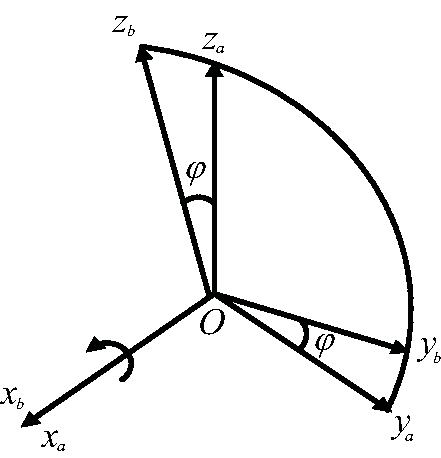
\includegraphics[width=0.77\linewidth]{pic/x}
		\vspace*{-0.5em}
		\caption{绕$x$轴旋转}
		\label{x}
	\end{minipage}
	\begin{minipage}{0.3\linewidth}
		\centering
		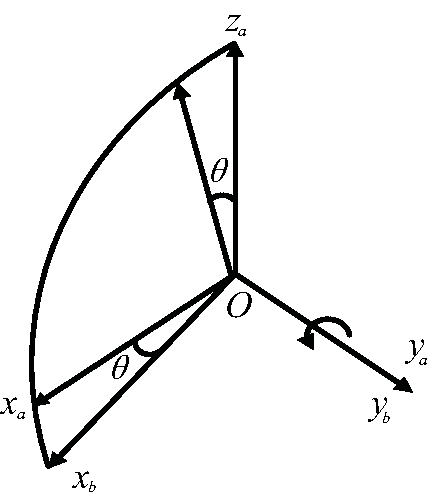
\includegraphics[width=0.78\linewidth]{pic/y}
		\vspace*{-0.5em}
		\caption{绕$y$轴旋转}
		\label{y}
	\end{minipage}
	\begin{minipage}{0.34\linewidth}
		\centering
		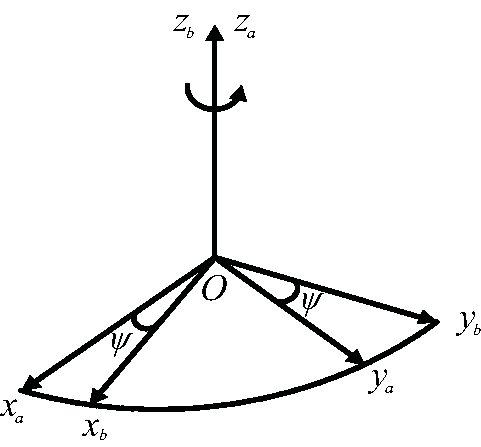
\includegraphics[width=0.85\linewidth]{pic/z}
		\vspace*{-0.5em}
		\caption{绕$z$轴旋转}
		\label{z}
	\end{minipage}
\end{figure}

下面给出两种基元旋转矩阵表示的坐标变换。
\vspace*{0.5em}

\sssection[$ZXZ$旋转顺序]

如图 \ref{ZXZ} 所示,方向余弦矩阵和$ZXZ$顺序欧拉角的关系为
\begin{equation}
	\bm{C}_{ba} = \bm{C}_z(\varphi) \bm{C}_x(\theta) \bm{C}_z(\psi) = 
	\begin{bmatrix}
		\cos \varphi \cos \psi - \sin \varphi \cos \theta \sin \psi & \cos \varpi \sin \psi + \sin \varphi \cos \theta \cos \psi & \sin \varphi \sin \theta \\
		- \sin \varphi \cos \psi - \cos \varphi \cos \theta \sin \psi & -\sin \varphi \sin \psi + \cos \varphi \cos \theta \cos \psi & \cos \varphi \sin \theta \\
		\sin \theta \sin \psi & -\sin \theta \cos \psi & \cos \theta 
	\end{bmatrix}
\end{equation}
通过与方向余弦矩阵的对应项进行对比,可以计算得到
\begin{equation}
	\begin{cases}
		\, \psi = -\tan^{-1}\left( \dfrac{C_{31}}{C_{32}} \right) \\
		\, \theta = \cos^{-1}\big( C_{33} \big) \\
		\, \varphi = \tan^{-1} \left( \dfrac{C_{13}}{C_{23}} \right)
	\end{cases}
	\label{eq:zxz}
\end{equation}
由公式 \eqref{eq:zxz} 可知,若欧拉角$\theta = 0\degree$,则欧拉转动处于奇异状态,欧拉角$\psi, \varphi$不能唯一确定。因此,$\theta$的取值范围为$0\degree<\theta<180\degree$。
\begin{figure}[!htb]
	\begin{minipage}{0.5\linewidth}
		\centering
		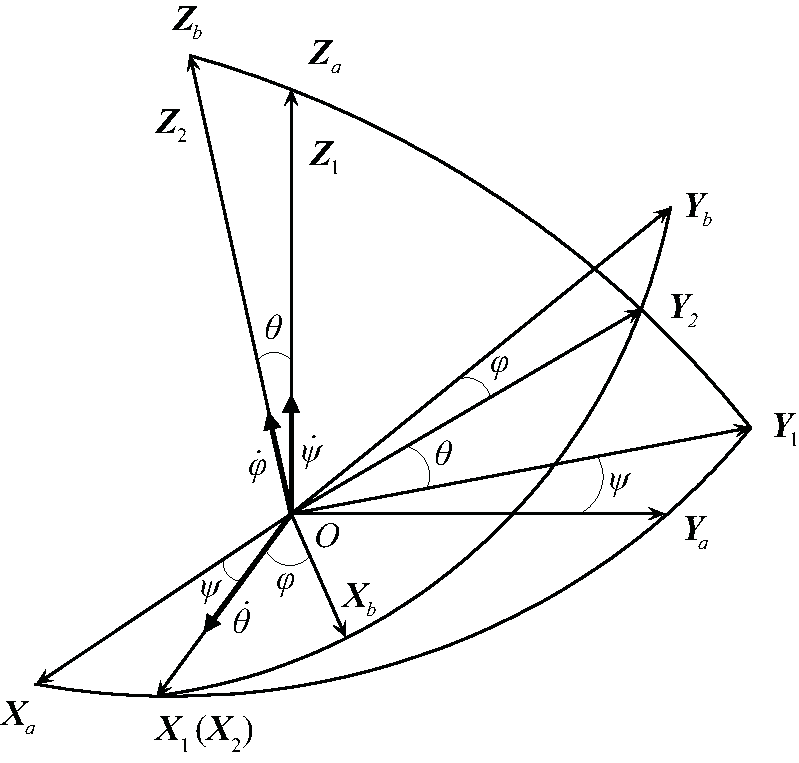
\includegraphics[width=0.8\linewidth]{pic/ZXZ}
		\vspace*{-1em}
		\caption{$ZXZ$顺序欧拉角旋转}
		\label{ZXZ}
	\end{minipage}
	\begin{minipage}{0.5\linewidth}
		\centering
		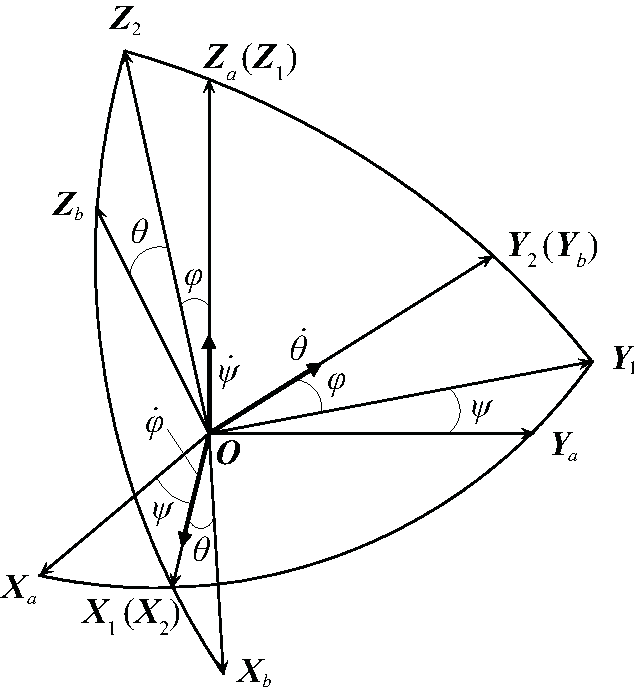
\includegraphics[width=0.695\linewidth]{pic/ZXY}
		\vspace*{-1em}
		\caption{$ZXY$顺序欧拉角旋转}
		\label{ZXY}
	\end{minipage}
\end{figure}


\sssection[$ZXY$旋转顺序]

如图 \ref{ZXY} 所示,方向余弦矩阵和$ZXY$顺序欧拉角的关系
\begin{equation}
	\bm{C}_{ba} = \bm{C}_y(\theta)\bm{C}_x(\varphi)\bm{C}_z(\psi) =
	\begin{bmatrix}
		\cos \theta \cos \psi - \sin \varphi \sin \theta \sin \psi & \cos \theta \sin \psi + \sin \varphi \sin \theta \cos \psi & -\cos \varphi \sin \theta \\
		-\cos \varphi \sin \psi & \cos \varphi \cos \psi & \sin \varphi \\
		\sin \theta \cos \varphi + \sin \varphi \cos \theta \sin \psi & \sin \theta \sin \psi - \sin \varphi \cos \theta \cos \psi & \cos \varphi \cos \theta 
	\end{bmatrix}
\end{equation}
通过与方向余弦矩阵的对应项进行对比,可以计算得到
\begin{equation}
	\begin{cases}
		\, \psi = -\tan^{-1}\left( \dfrac{C_{21}}{C_{22}} \right) \\
		\, \theta = \sin^{-1}\big( C_{23} \big) \\[0.5em]
		\, \varphi = \tan^{-1} \left( \dfrac{C_{13}}{C_{33}} \right)
	\end{cases}
	\label{eq:zxy}
\end{equation}

由公式 \eqref{eq:zxy} 可知,若欧拉角$\theta = \pm 90 \degree$,则欧拉转动处于奇异状态,欧拉角$\psi, \varphi$在同一平面转动,不能唯一确定。
\vspace*{0.5em}



\section{欧拉轴角}
\label{sec: 欧拉轴角}
\vspace*{-1.5em}

\defination{欧拉轴 / 角}
{
	坐标系$S_b$相对坐标系$S_a$的姿态参数可以用单位矢量$\bm{e}$在参考坐标系$S_a$的三个分量$e_x, e_y, e_z$以及绕此转轴的转角$\varPhi$这4个参数来描述,称为\dy{欧拉轴 / 角}{OLZJ}参数。矢量$\bm{e}$称为\dy{欧拉轴}{OLZ},$\varPhi$称为\dy{欧拉转角}{OLZJ}。
}

\subsection{欧拉轴 / 角与方向余项矩阵的相互转换}

\sssection[欧拉轴 / 角求方向余弦矩阵]

方向余项矩阵$\bm{C}_{ba}$可由欧拉轴 / 角参数$\bm{e}, \varPhi$得到。
\begin{figure}[!htb]
	\begin{minipage}{0.31\linewidth}
		\centering
		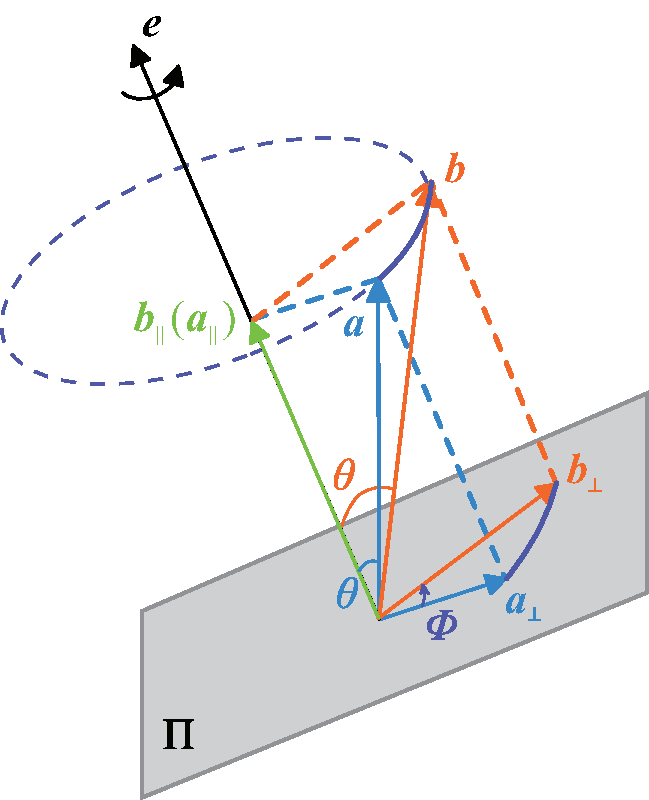
\includegraphics[width=0.9\linewidth]{pic/欧拉轴}
		\vspace*{-1.2em}
		\caption{欧拉轴旋转分解图}
		\label{欧拉轴}
	\end{minipage}
	\begin{minipage}{0.33\linewidth}
		\centering
		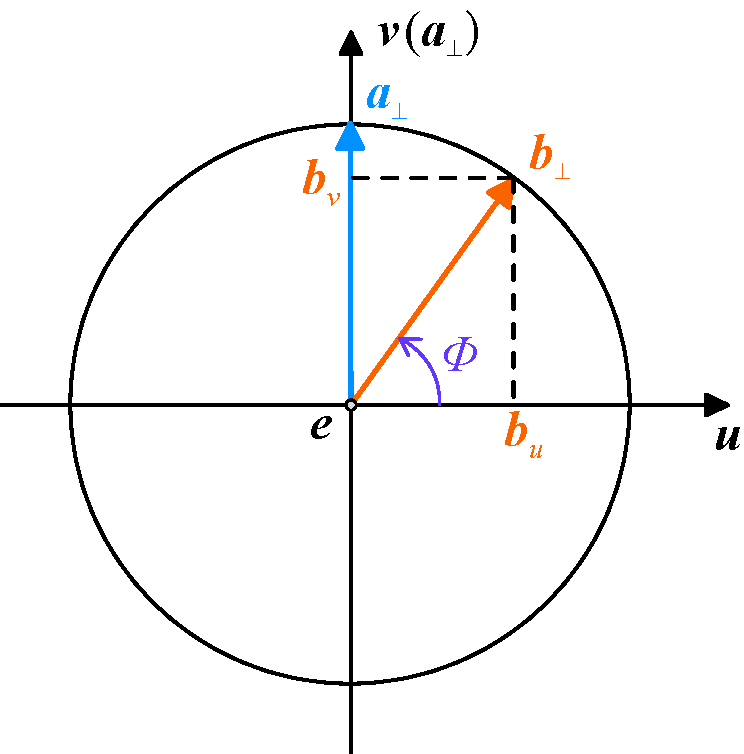
\includegraphics[width=\linewidth]{pic/欧拉轴2}
        \vspace*{-2.6em}
		\caption{欧拉轴旋转投影图}
		\label{欧拉轴2}
	\end{minipage}
	\begin{minipage}{0.33\linewidth}
		\centering
		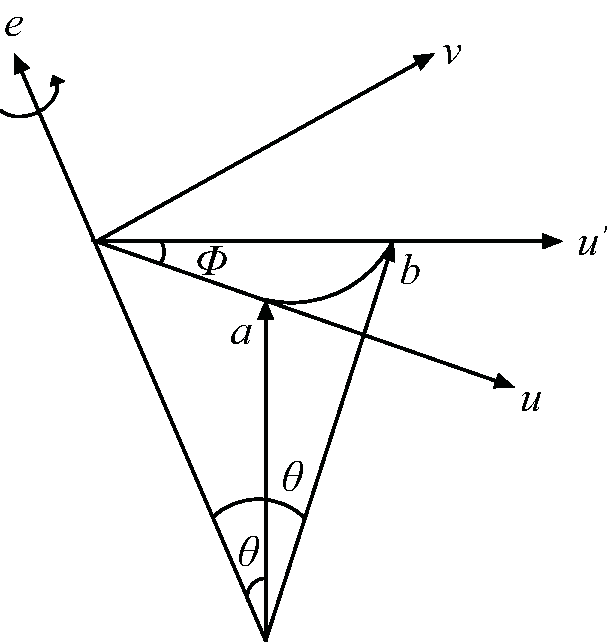
\includegraphics[width=0.913\linewidth]{pic/欧拉轴角}
		\caption{欧拉轴 / 角的坐标变换图}
		\label{欧拉轴角}
	\end{minipage}
\end{figure}

如图 \ref{欧拉轴} 所示,设矢量$\bm{a}$是固定在坐标系$S_a$的任意矢量,矢量$\bm{b}$是固定于坐标系$S_b$中的矢量。将矢量$\bm{a}$绕轴$\bm{e}$旋转一个角度$\varPhi$后得到矢量$\bm{b}$。首先将矢量$\bm{a}$,矢量$\bm{b}$沿轴$\bm{e}$方向和垂直于轴$\bm{e}$方向分解,其平行分量$\bm{a}_{\parallel} = \bm{b}_{\parallel} = \bm{e}$相等,即旋转前后不变,可以发现旋转仅与垂直分量$\bm{a}_{\perp}, \bm{b}_{\perp}$有关。

将垂直分量$\bm{a}_{\perp}, \bm{b}_{\perp}$投影到垂直于轴$\bm{e}$的平面$\Pi$上,如图 \ref{欧拉轴2} 所示。定义单位正交矢量$\bm{u}, \bm{v}$
\begin{align*}
	\bm{v} & = \bm{a}_{\perp} = \dfrac{\bm{e} \times \bm{a}}{\big| \bm{e} \times \bm{a} \big|} = \dfrac{1}{a \sin \theta}(\bm{e} \times \bm{a}) \\
	\bm{u} & = \bm{v} \times \bm{e} = \dfrac{1}{a \sin \theta} (\bm{e} \times \bm{a}) \times \bm{e} = \dfrac{1}{a \sin \theta}\big[ \bm{a} - (\bm{e} \cdot \bm{a})\bm{e} \big] 
\end{align*}
将矢量$\bm{b}_{\perp}$分解,得
\begin{equation*}
	\bm{b}_{\perp} = \cos \varPhi \bm{u} + \sin \varPhi \bm{v} = \cos \varPhi (\bm{a}_\perp \times \bm{e}) + \sin \varPhi \bm{a}_\perp
\end{equation*}
将矢量$\bm{a}, \bm{b}$用上面的矢量表示为(注:$\bm{a}, \bm{b}$模长相等,即$a=b$)
\begin{align}
	\bm{a} & = a \big( \cos \theta \bm{a}_{\parallel} + \sin \theta \bm{a}_{\perp} \big) 
	= a \big( \cos \theta \bm{e} + \sin \theta \bm{v} \big) \\
	\bm{b} & = b \big( \cos \theta \bm{b}_{\parallel} + \sin \theta \bm{b}_{\perp} \big) 
	= a \big( \cos \theta \bm{e} + \sin \theta \bm{b}_{\perp} \big)
\end{align}
将$\bm{b}_{\perp}$的表达式反代,可以得到
\begin{equation}
	\bm{b} = \cos \varPhi \bm{a} + ( 1 - \cos \varPhi ) (\bm{e} \cdot \bm{a})\bm{e} + \sin \varPhi(\bm{e} \times \bm{a})
\end{equation}
为了写成矩阵形式,我们利用把向量(在坐标系$S_a$的分量)的计算转换为矩阵的形式\footnote[1]{关于$\bm{e}\bm{e}^\T$和叉乘矩阵$\bm{e}^\times$的说明及向量运算矩阵表示的证明,详见前面的小节: \ref{向量运算的矩阵表示} \link[向量运算的矩阵表示]},即
\begin{align*}
	\bm{e} \cdot \bm{a} \cdot \bm{e} = 
	\big[ \bm{i}_a \quad \bm{j}_a \quad \bm{k}_a \big] \,
	\begin{bmatrix}
		e_x \\
		e_y \\
		e_z
	\end{bmatrix}
	\,
	\big[ e_x \quad e_y \quad e_z \big]
	\,
	\begin{bmatrix}
		a_x \\
		a_y \\
		a_z
	\end{bmatrix}
	= \bm{e}_a^\T \bm{e} \bm{e}^\text{T} \bm{a},
	&& \bm{e} \times \bm{a} =
	\big[ \bm{i}_a \quad \bm{j}_a \quad \bm{k}_a \big] \,
	\begin{bmatrix}
		0 & -e_z & e_y \\
		e_z & 0 & -e_x \\
		-e_y & e_x & 0
	\end{bmatrix}
	\,
	\begin{bmatrix}
		a_x \\
		a_y \\
		a_z
	\end{bmatrix}
	= \bm{e}_a^\T \bm{e}^\times \bm{a}
\end{align*}
将$\bm{a}, \bm{b}$在坐标系$S_a$下分解,得
\begin{equation}
	\bm{e}_a^\T \bm{b} = \cos \varPhi \bm{e}_a^\T\bm{a} + ( 1 - \cos \varPhi ) \bm{e}_a^\T \bm{e} \bm{e}^\text{T} \bm{a} + \sin \varPhi \bm{e}_a^\T \bm{e}^\times \bm{a}
\end{equation}
两边同时左乘$\big[ \bm{e}_a^\T \big]^{-1}$,消去$\bm{e}_a^\T$,可以得到
\begin{align}
	\bm{b} &= \cos \varPhi \bm{a} + (1 - \cos \varPhi)\bm{e}\bm{e}^\T \bm{a} + \sin \varPhi \bm{e}_a^\T \bm{e}^ \times \bm{a} \notag \\
	& = \big[ \cos \varPhi \bm{E}_3 + (1 - \cos \varPhi) \bm{e} \bm{e}^\T + \sin \varPhi \bm{e}_a^\T \bm{e}^ \times \big] \bm{a}
\end{align}
可以得到

\theorem{欧拉轴 / 角参数下的向量旋转矩阵}
{
	在同一坐标系$S_a$下将向量$\bm{a}$绕轴$\bm{e}$旋转$\varPhi$角度得到向量$\bm{b}$,它们的关系为
	\begin{equation}
		\bm{b} = \bm{R}_{ba} \bm{a}
	\end{equation}
	其中,\dy{向量旋转矩阵}{XLXZJZ}定义为
	\begin{align}
		\bm{R}_{ba} 
		& = \cos \varPhi \bm{E}_3 + \big( 1 - \cos \varPhi \big) \bm{e} \bm{e}^\T + \sin \varPhi \bm{e}^{\times} \\
		& = 
		\begin{bmatrix}
			\cos \varPhi + e_x^2 \big( 1 - \cos \varPhi \big) & e_x e_y \big( 1 - \cos \varPhi \big) - e_z \sin \varPhi & e_x e_z \big( 1 - \cos \varPhi \big) + e_y \sin \varPhi \\
			e_x e_y \big( 1 - \cos \varPhi \big) + e_z \sin \varPhi & \cos \varPhi + e_y^2 \big( 1 - \cos \varPhi \big) & e_y e_z \big(1 - \cos \varPhi \big) - e_x \sin \varPhi \\
			e_x e_z \big( 1 - \cos \varPhi \big) - e_y \sin \varPhi & e_y e_z \big( 1- \cos \varPhi \big) + e_x \sin \varPhi & \cos \varPhi + e_z^2 \big( 1- \cos \varPhi \big)
		\end{bmatrix}
		\nomenclature{$\bm{R}_{ba}$}{坐标系$S_a$中的向量分量变换到坐标系$S_b$的旋转矩阵  \nomrefpage}
	\end{align}
}

而由向量旋转与坐标系旋转的对应关系,可以知道向量旋转矩阵和坐标系旋转矩阵(方向余弦矩阵)互为转置(逆),所以可以得到\footnote[2]{证明详见 第 \ref{参考内容} 章 : \ref{向量旋转矩阵和坐标系旋转矩阵的关系} \link[向量旋转矩阵和坐标系旋转矩阵的关系]}

\theorem{欧拉轴 / 角参数下的坐标系旋转矩阵(方向余弦矩阵)}
{
	欧拉轴 / 角参数下的坐标系旋转矩阵(方向余弦矩阵)为
	\begin{align}
		\bm{C}_{ba} & = (\bm{R}_{ba})^\T 
		= \big[\cos \varPhi \bm{E}_3 + \big( 1 - \cos \varPhi \big) \bm{e} \bm{e}^\T + \sin \varPhi \bm{e}^{\times}\big]^\T \notag \\
		& = \cos \varPhi \bm{E}_3 + \big( 1 - \cos \varPhi \big) (\bm{e} \bm{e}^\T)^\T + \sin \varPhi (\bm{e}^{\times})^\T \notag \\
		& = \cos \varPhi \bm{E}_3 + \big( 1 - \cos \varPhi \big) \bm{e} \bm{e}^\T - \sin \varPhi \bm{e}^\times \\
		& = 
		\begin{bmatrix}
			\cos \varPhi + e_x^2 \big( 1 - \cos \varPhi \big) & e_x e_y \big( 1 - \cos \varPhi \big) + e_z \sin \varPhi & e_x e_z \big( 1 - \cos \varPhi \big) - e_y \sin \varPhi \\
			e_x e_y \big( 1 - \cos \varPhi \big) - e_z \sin \varPhi & \cos \varPhi + e_y^2 \big( 1 - \cos \varPhi \big) & e_y e_z \big(1 - \cos \varPhi \big) + e_x \sin \varPhi \\
			e_x e_z \big( 1 - \cos \varPhi \big) + e_y \sin \varPhi & e_y e_z \big( 1- \cos \varPhi \big) - e_x \sin \varPhi & \cos \varPhi + e_z^2 \big( 1- \cos \varPhi \big)
		\end{bmatrix}
		\nomenclature{$\bm{E}_i$}{$i \times i$的单位矩阵 \nomrefpage}
	\end{align}
}


\sssection[由方向余弦矩阵确定欧拉轴 / 角参数]

若已知方向余弦矩阵$\bm{C}_{ba}$,可以计算得到欧拉轴 / 角参数,得
\begin{align}
	\cos \varPhi = \dfrac{\text{tr} \bm{C}_{ba} - 1}{2} \\
	\bm{e} = \dfrac{1}{2 \sin \varPhi} 
	\begin{bmatrix}
		C_{23} - C_{32} \\
		C_{31} - C_{13} \\
		C_{12} - C_{21}
	\end{bmatrix}
\end{align}
其中,$\text{tr} \bm{C}_{ba}$是方向余弦矩阵的迹,$\text{tr} \bm{C}_{ba} = C_{11} + C_{22} + C_{33}$。绕任意轴转动相同的$\varPhi$角,方向余项矩阵的迹不变。

\noindent 将公式展开,对应得到以下3组解:

\noa[1] 当$\text{tr} \bm{C}_{ba} \neq 3, -1$时,可以直接计算分量$e_x, e_y, e_z$。

\noa[2] 当$\text{tr} \bm{C}_{ba} = 3$时,此时对应转角$\varPhi = 0, \pm 2 \pi, \pm 4 \pi, \cdots$,方向余弦矩阵$\bm{C}_{ba}$为单位矩阵,$e_x, e_y, e_z$无法确定。这种情况相当于没有发生转动。

\noa[3] 当$\text{tr} \bm{C}_{ba} = -1$时,对应转角$\varPhi = \pm \pi, \pm 3 \pi, \pm 5 \pi, \cdots$,此时$\bm{C}_{ba} = 2 \bm{e}\bm{e} - \bm{E}_3$,则有
\begin{equation}
	\begin{cases}
		\, e_x = \pm \sqrt{\dfrac{1 + C_{11}}{2}}, \qquad e_y = \pm \sqrt{\dfrac{1+ C_{22}}{2}}, \qquad e_z = \pm \sqrt{\dfrac{1 + C_{33}}{2}} \\[0.5em]
		\, e_x e_y = \dfrac{1}{2} C_{12}, \hspace*{3.7em} e_ye_z = \dfrac{1}{2}C_{23}, \hspace*{3.7em} e_ze_x = \dfrac{1}{2} C_{31}
	\end{cases}
\end{equation}
其中,使用后三个方程来判断前三个方程的符号。

\begin{figure}[!htb]
	\centering
	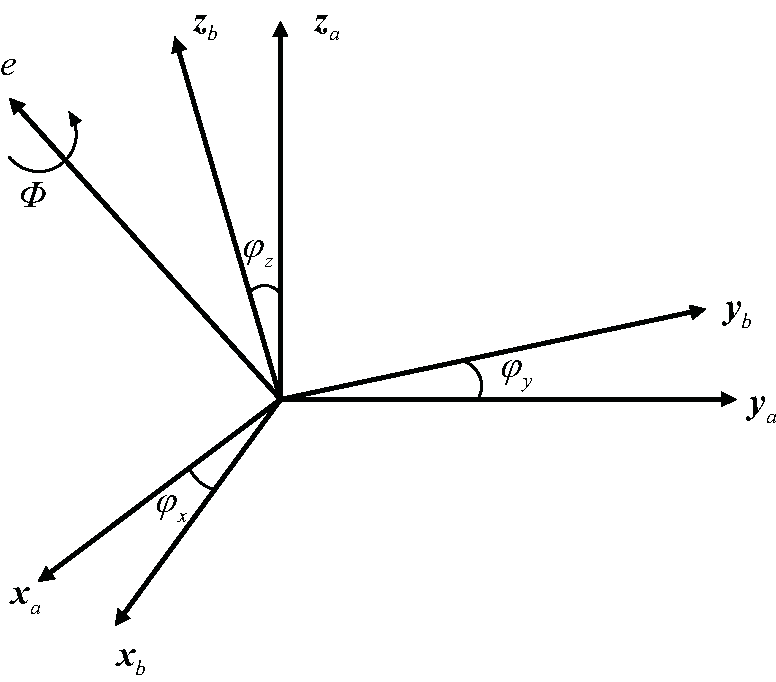
\includegraphics[width=0.42\linewidth]{pic/欧拉轴角变换}
	\vspace*{-1em}
	\caption{欧拉转角与两个坐标系之间的几何关系}
	\label{欧拉转角变换}
\end{figure}
\vspace*{-1.8em}

\subsection{欧拉转角的几何意义}

如图 \ref{欧拉转角变换} 所示,令$\varphi_x, \varphi_y, \varphi_z$分别为两个坐标系对应轴之间的夹角,方向余弦矩阵的对焦线上的元素即为这几个角的余弦值,所以
\begin{equation}
	2 \cos \varPhi = \text{tr} \bm{C}_{ba} - 1 = \cos \varphi_x + \cos \varphi_y + \cos \varphi_z - 1
\end{equation}
利用半角公式$\cos \alpha = 1 - 2 \sin^2 \dfrac{\alpha}{2}$,则
\begin{equation}
	\sin^2 \dfrac{\varPhi}{2} = \dfrac{1}{2} \left( \sin^2 \dfrac{\varphi_x}{2} + \sin^2 \dfrac{\varphi_y}{2} + \sin^2 \dfrac{\varphi_z}{2} \right)
\end{equation}

当偏角较小时,有
\begin{equation}
	\varPhi \approx \dfrac{\sqrt{2}}{2} \sqrt{\varphi_x^2 + \varphi_y^2 + \varphi_z^2}
\end{equation}
这个公式对于评价旋转误差是很有用的。
\vspace*{1em}



\section{四元数}
\subsection{四元数的定义}

\defination{四元数}
{
	\dy{四元数}{SYS}的定义和复数类似,唯一的区别就是四元数一共有三个虚部,而复数只有一个。所有的四元数$q \in \mathbb{H}$($\mathbb{H}$代表四元数的发现者 William Rowan Hamilton)都可以写成下面这种形式
	\vspace*{-0.7em}
	\begin{equation}
		q = a + b i + cj +dk \quad (a,b,c,d \in \mathbb{R})
		\nomenclature{$q$}{四元数 \nomrefpage}
		\vspace*{-0.7em}
	\end{equation}
	其中,
	\vspace*{-0.7em}
	\begin{equation}
		i^2 = j^2 = k^2 = i j k = -1
	\end{equation}
}

四元数可以写成向量形式
\begin{equation}
	q = 
	\begin{bmatrix}
		a \\
		b \\
		c \\
		d
	\end{bmatrix}
\end{equation}
同时,通常将四元数的实部与虚部分开,并用一个三维的向量来表示虚部,将它表示为\dy{标量向量有序对}{BLXLYXD}形式
\begin{equation}
	q = \big[ s, \bm{v} \big],
	\quad 
	\bm{v} = 
	\begin{bmatrix}
		x \\
		y \\
		z
	\end{bmatrix} 
	\quad (s,x,y,z \in \mathbb{R})
\end{equation}

\subsection{四元数的基本运算}

\sssection[四元数的模长]
\vspace*{-0.5em}

\defination{四元数的模长}
{
	\dy{四元数的模长}{SYSDMC}(范数)定义为
	\begin{equation}
		\norm[q] = \sqrt{a^2 + b^2 + c^2 + d^2}
		\nomenclature{$\norm[q]$}{四元数的模长(范数)}
	\end{equation}
	用标量向量有序对表示为
	\begin{equation}
		\norm[q] = \sqrt{s^2 + \norm[\bm{v}]^2} = \sqrt{s^2 + \bm{v} \cdot \bm{v}}
	\end{equation}
	\textbf{注:由于四元数是四维向量,其没有明确的物理几何意义。}
}


\sssection[四元数的加减运算]

四元数的加减运算和复数一致,设两个四元数为$q_1 = a + bi + cj + dk,\, q_2 = e + fi +gj + hk$,则
\begin{align}
	q_1 \pm q_2 & = a + bi + cj + dk \pm (e + fi +gj + hk) \notag \\
	& = (a \pm e)  + (b \pm f) i + (c \pm g) j + (d \pm h) k
\end{align}
标量向量对形式的加减与标量和向量的加减运算一致,设两个四元数为$q_1 = \big[s, \bm{v}\big],\, q_2 = \big[ t, \bm{u} \big]$,则
\begin{equation}
	q_1 \pm q_2 = \big[ s \pm t, \bm{v} \pm \bm{u} \big]
\end{equation}


\sssection[四元数的数乘]

一个四元数$q = a +bi +cj +dk$和标量$s$的乘积为
\begin{align}
	sq &= s (a + bi +cj +dk) \notag \\
	& = sa + sbi +scj +sdk
\end{align}
四元数的数乘运算满足交换律,即$sq = qs$.
\vspace*{1em}


\sssection[四元数的乘法]

四元数的乘法和矩阵乘法类似,不遵守交换律,即在一般情况下$q_1 q_2 \neq q_2 q_1$。所以,四元数乘法和矩阵乘法一样有左乘和右乘的区别。即

\noa[1] $q_1 q_2$\quad $q_1\,$\dy{左乘}{ZC}$\,q_2$\quad 或\quad $q_2\,$\dy{右乘}{YC}$\,q_1$.

\noa[2] $q_2 q_1$\quad $q_1\,$\dy{右乘}{YC}$\,q_2$\quad 或\quad $q_2\,$\dy{左乘}{ZC}$\,q_1$.

四元数的乘法满足结合律和分配律。

那么,如果有两个四元数$q_1 = \big[s, \bm{v}\big],\, q_2 = \big[ t, \bm{u} \big]$,则
\begin{align}
	q_1 q_2 & = (a + bi +cj +dk)(e + fi +gj +hk) \notag  \\
	& = ae + afi + agj + ak \notag \\
	& + bei + bfi^2 + bgij + bhik \notag \\
	& + cej + cfji + cgj^2 + chjk \notag \\
	& + dek + dfki + dgkj + dhk^2
\end{align}
利用四元数的性质$i^2 = j^2 = k^2 = i j k = -1$,可以得到
\begin{align}
	 ijk = -1 \, &\xrightarrow{\quad \textstyle \mbox{等式两边同时左乘} \,\, i \quad } \, iijk = -i \hspace*{-8em} &&\Rightarrow \quad jk = i \\
	 ijk = -1 \, &\xrightarrow{\quad \textstyle \mbox{等式两边同时右乘} \,\, k \quad } \, ijkk = -k \hspace*{-8em} &&\Rightarrow \quad ij = k \\
	 jk = i \, &\xrightarrow{\quad \textstyle \mbox{等式两边同时左乘} \,\, j \quad } \, jjk = ji  \hspace*{-8em} &&\Rightarrow \quad ji = -k \\
	 jk = i \, &\xrightarrow{\quad \textstyle \mbox{等式两边同时右乘} \,\, k \quad } \, jkk = ik  \hspace*{-8em} &&\Rightarrow \quad ik = -j \\
	 ij = k \, &\xrightarrow{\quad \textstyle \mbox{等式两边同时左乘} \,\, i \quad } \, iij = ik \hspace*{-8em} &&\Rightarrow \quad ik = -j \\
	 ij = k \, &\xrightarrow{\quad \textstyle \mbox{等式两边同时右乘} \,\, j \quad } \, ijj = kj \hspace*{-8em} &&\Rightarrow \quad kj = -i
\end{align}
将上面的性质整理为表格如表 \ref{四元数基本乘法} 所示。
\begin{table}[!htb]
	\centering
	\setlength{\tabcolsep}{2em}{
	\begin{tabular}{|c|c|c|c|c|}
		\hline
		\rowcolor{Azure2} $\times$ & 1 & $ i $ & $ j $ & $ k $ \\
		\hline
		\cellcolor{Azure2} 1 & 1 & $i$ & $j$ & $k$ \\
		\hline
		\cellcolor{Azure2} $i$ & $i$ & $-1$ &\cellcolor{MistyRose} $k$ & \cellcolor{DarkSlateGray2} $-j$ \\
		\hline
		\cellcolor{Azure2} $j$ & $j$ & \cellcolor{MistyRose} $-k$ & $-1$ & \cellcolor{LightGoldenrod1} $i$ \\
		\hline
		\cellcolor{Azure2} $k$ & $k$ & \cellcolor{DarkSlateGray2} $j$ &  \cellcolor{LightGoldenrod1} $-i$ & $-1$ \\
		\hline
	\end{tabular}
}
\caption{四元数基本向量的乘法计算表(左$\times$上)}
\label{四元数基本乘法}
\end{table}
\vspace*{-2em}

\summarize[
\hspace{1em} 记忆方法:类似于向量的叉乘,将$i,j,k$理解为三维右手坐标系,则$i \times j =k , j \times i = -k$,其余类似。
]

利用表 \ref{四元数基本乘法} ,可以将四元数乘法的结果化简为
\begin{align}
	q_1 q_2 & = ae + afi + agj + ak \notag \\
& + bei + bfi^2 + bgij + bhik \notag \\
& + cej + cfji + cgj^2 + chjk \notag \\
& + dek + dfki + dgkj + dhk^2 \notag \\
& = (a {\color{VioletRed} e} - b {\color{cyan} f} - c{\color{SeaGreen} g} - d{\color{orange} h}) \notag \\
& + (b {\color{VioletRed} e} - a {\color{cyan} f} - d{\color{SeaGreen} g} - c{\color{orange} h}) i \notag \\
& + (c {\color{VioletRed} e} - d {\color{cyan} f} - a{\color{SeaGreen} g} - b{\color{orange} h}) j \notag \\
& + (d {\color{VioletRed} e} - c {\color{cyan} f} - b{\color{SeaGreen} g} - a{\color{orange} h}) k
\end{align}
写成矩阵为
\begin{equation}
		q_1 q_2 = 
		\begin{bmatrix}
			a & -b & -c & -d \\
			b & a & -d & c \\
			c & d & a & -b \\
			d & -c & b & a
		\end{bmatrix}
		\,\, 
		\begin{bmatrix}
		 {\color{VioletRed} e} \\
		 {\color{cyan} f} \\
		 {\color{SeaGreen} g} \\
		 {\color{orange} h} 
		\end{bmatrix}
\end{equation}
同理可得,右乘的结果为
\begin{equation}
	q_2 q_1 = 
	\begin{bmatrix}
		a & -b & -c & -d \\
		b & a & d & c \\
		c & -d & a & b \\
		d & c & -b & a
	\end{bmatrix}
	\,\, 
	\begin{bmatrix}
		{\color{VioletRed} e} \\
		{\color{cyan} f} \\
		{\color{SeaGreen} g} \\
		{\color{orange} h} 
	\end{bmatrix}
\end{equation}
\vspace*{0.5em}


\sssection[Grassmann 积]

为了将四元数的结果写成标量向量有序对,重新整理结果
\begin{align}
	q_1 q_2 & = (ae - ({\color{SeaGreen}bf + cg + dh})) \notag \\
	& + (b {\color{VioletRed} e} + {\color{cyan} a}f +{\color{orange} ch - dg} ) i \notag \\
	& + (c {\color{VioletRed} e} + {\color{cyan} a}g +{\color{orange} df - bh} ) j \notag \\
	& + (d {\color{VioletRed} e} + {\color{cyan} a}h +{\color{orange} bg - cf} ) k \notag 
\end{align}
令
$
\bm{v} = 
\begin{bmatrix}
	b \\
	c \\
	d
\end{bmatrix}
, \,
\bm{u} = 
\begin{bmatrix}
	f \\
	g \\
	h
\end{bmatrix}
$,那么
\begin{align*}
	\bm{v} \cdot \bm{u} &= {\color{SeaGreen}bf + cg + dh} \\
	\bm{v} \times \bm{u} &= 
	\begin{vmatrix}
		\bm{i} & \bm{j} & \bm{k} \\
		b & c & d \\
		f& g & h
	\end{vmatrix}
= ({\color{orange} ch - dg}) \bm{i} + ({\color{orange} df - bh} )\bm{j} + ({\color{orange} bg - cf} )\bm{k}
\end{align*}
所以,$q_1q_2$的结果可以用向量点乘和叉乘的形式表示出来\footnote[1]{其实按照历史的顺序来说,这里第一次提出叉乘的概念。}
\begin{equation}
	q_1 q_2 = \big[ ae - \bm{v} \cdot \bm{u}, a\bm{u} +e \bm{v} + \bm{v} \times \bm{u} \big]
\end{equation}

这个结果称为\dy{Grassmann积}{GRASSMANNJ},一般来说

\theorem{Grassmann 积}
{
	对于任意四元数$q_1= \big[s, \bm{v} \big],\, q_2= \big[ t, \bm{u} \big]$,$q_1q_2$的结果为
	\begin{equation}
		q_1 q_2 = \big[ st - \bm{v} \cdot \bm{u}, s \bm{u} + t \bm{v} + \bm{v} \times \bm{u} \big]
		\label{Grassmann}
	\end{equation}
}
\vspace*{0.5em}


\sssection[四元数的逆]

因为四元数不遵守交换律,所以类似于矩阵除法,四元数相除等价于乘以它的逆。同样地,也有左除和右除之分,即$pq^{-1}$或$q^{-1}p$,它们的结果一般不同。


\defination{四元数的逆}
{
	如果
	\begin{equation}
		qq^{-1} = q^{-1} q = 1 \quad (q \neq 0)
		\nomenclature{$q^{-1}$}{四元数的逆 \nomrefpage}
	\end{equation}
	那么,我们称$q^{-1}$为四元数$q$的\dy{逆}{N}。
}

直接求解一个四元数的逆$q^{-1}$是非常困难的,但是我们可以使用四元数共轭的性质来求$q^{-1}$。
\vspace*{1em}


\sssection[共轭四元数]
\vspace*{-0.5em}

\defination{共轭四元数}
{
	一个四元数$q = a + bi + cj + dk$的\dy{共轭}{GE}为
	\begin{equation}
		q^* = a - bi - ci -dk
		\nomenclature{$q^*$}{四元数$q$的共轭 \nomrefpage}
	\end{equation}
	如果用标量向量有序对的形式来定义,则$q = \big[ s, \bm{v} \big]$的\dy{共轭}{GE}为
	\begin{equation}
		q^* = \big[ s, -\bm{v} \big]
	\end{equation}
}

共轭四元数的一个非常有用的性质就是
\begin{align}
	q q^* &= \big[s, \bm{v}] \cdot \big[s, - \bm{v}] \notag \\
	& = \big [s^2 - \bm{v} \cdot \bm{v}, s(- \bm{v}) + s \bm{v} + \bm{v} \times (- \bm{v})] \notag \\
	& = \big[s^2 + \bm{v}\cdot \bm{v}, 0] \notag \\
	& = s^2 + x^2 + y^2 + z^2 = \norm[q]^2 \quad \left(\bm{v} = \big[ x, y, z \big]\right) 
\end{align}
因为$(q^*)^* = \big [s, - (- \bm{v})] = \big[s, \bm{v}\big] = q$,则
\begin{equation}
	q^* q = (q^*)(q^*)^* = \norm[q^*]^2 = s^2 + x^2 +y^2 + z^2 = \norm[q]^2 = q q^* 
\end{equation}
这说明,$q^*q = qq^*$。这个特殊的乘法是遵守交换律的。

下面利用四元数的性质求四元数的逆。
\begin{align*}
	q q^{-1} = 1 \, \xrightarrow{\textstyle \quad \mbox{等式两边同时左乘}\, q^* \quad }\, q^* q q^{-1} = 1 &\quad \Rightarrow \quad (q^* q)q^{-1} = q^* \, \xrightarrow{\quad \textstyle q^* q = \norm[q]^2 \quad } \norm[q]^2 \cdot q^{-1} = q^* \notag
\end{align*}
由此可知

\theorem{四元数逆的求解}
{
	四元数的逆可以表示为
	\begin{equation}
		q^{-1} = \dfrac{q^*}{\norm[q]^2}
	\end{equation}
	用这种方法寻找一个四元数的逆会非常高效,我们只需要将一个四元数的共轭除以它的模长的平方就可以得到四元数的逆。特别地对于\dy{单位四元数}{DWSYS}$\norm[q] = 1$来说,它的逆为
	\begin{equation}
		q^{-1} = \dfrac{q^*}{1^2} = q^*
	\end{equation}
}


\sssection[纯四元数]
\vspace*{-0.5em}

\defination{纯四元数}
{
	如果一个四元数实部为0,仅有虚部,即
	\begin{equation}
		v = \big[ 0, \bm{v} \big]
	\end{equation}
	那么我们则称这个四元数$v$为一个\dy{纯四元数}{CXYS}。因为纯四元数仅由虚部的三维向量决定,我们可以将任意的三维向量转换为纯四元数。
}

纯四元数有一个很重要的特性:两个纯四元数$v = \big[ 0, \bm{v} \big], u = \big[ 0, \bm{u} \big]$的乘积为
\begin{align}
	vu &= \big[ 0 - \bm{v} \cdot \bm{u}, 0 + \bm{v} \times \bm{u} \big]  = \big[ - \bm{v} \cdot \bm{u}, \bm{v} \times \bm{u} \big]
	\label{eq: 纯四元数乘法}
\end{align}


\subsection{四元数与三维旋转}

\begin{figure}[!htb]
	\centering
	\begin{minipage}{0.31\linewidth}
		\centering
		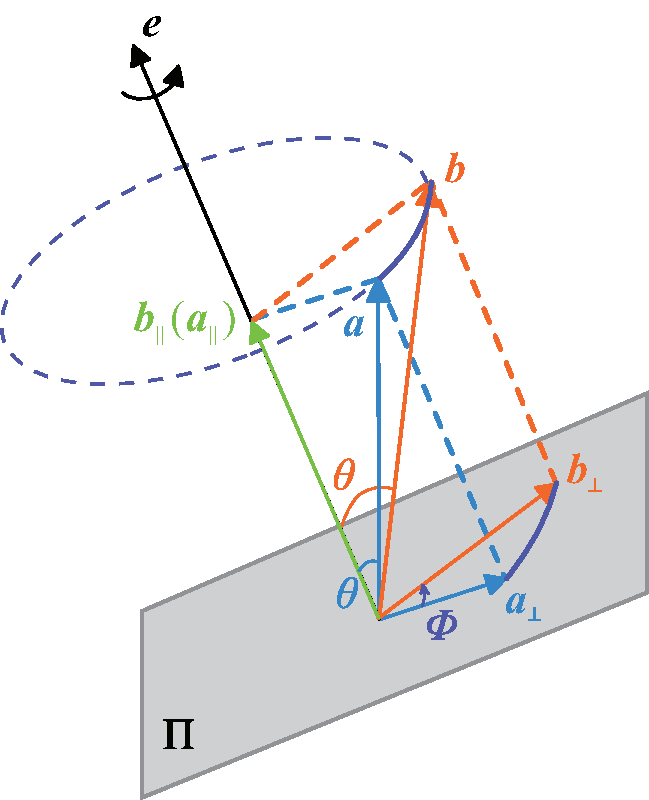
\includegraphics[width=0.9\linewidth]{pic/欧拉轴}
		\vspace*{-1.2em}
		\caption{向量旋转分解图}
		\label{欧拉轴3}
	\end{minipage}\hspace*{7em}
	\begin{minipage}{0.348\linewidth}
		\centering
		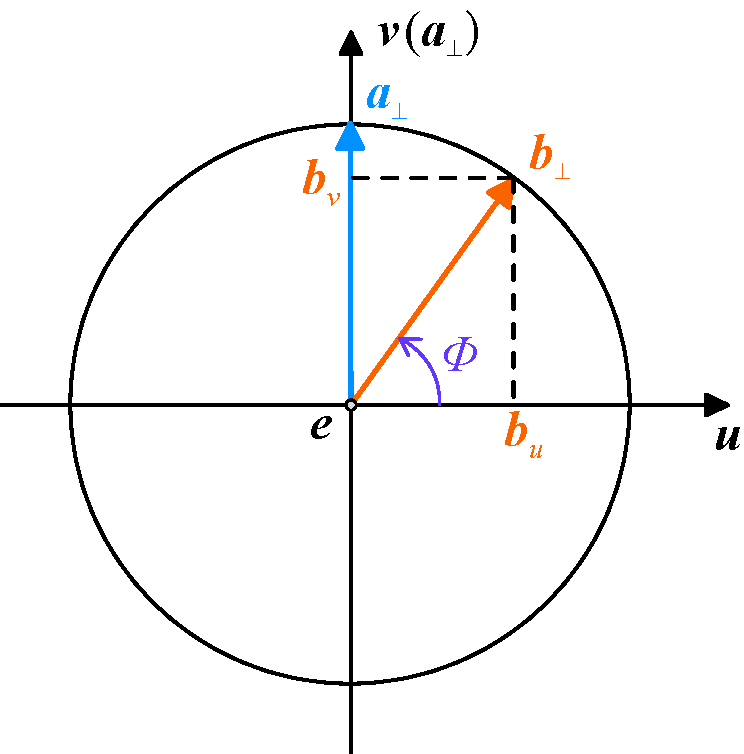
\includegraphics[width=\linewidth]{pic/欧拉轴2}
		\caption{向量旋转投影图}
		\label{欧拉轴4}
	\end{minipage}
\end{figure}

在上个章节 \ref{sec: 欧拉轴角} 中我们知道:如果我们需要将一个向量$\bm{a}$沿着一个用单位向量$\bm{e}$所定义的旋转轴旋转$\varPhi$度,那么我们可以将这个向量$\bm{a}$可以分解为平行于旋转轴的分量$a_{\parallel}$和垂直于旋转轴的分量$a_{\perp}$。旋转后得到的向量$\bm{b}$可以表示为这两个分量分别旋转后之和,即$\bm{b} = \bm{b}_{\parallel} + \bm{b}_{\perp}$。

我们定义这些向量为纯四元数
\begin{align*}
	a &= \big[ 0, \bm{a} \big]  && b = \big[ 0, \bm{b} \big] \\
	a_\perp &= \big[ 0, \bm{a}_\perp \big] && b_\perp = \big[ 0, \bm{b}_\perp \big] \\
	a_\parallel &= \big[ 0, \bm{a}_\parallel \big] && b_\parallel = \big[ 0, \bm{b}_\parallel \big] \\
	e &= \big[0, \bm{e} \big] 
\end{align*}
那么我们可以得到
\begin{equation*}
	a = a_\parallel + a_\perp \qquad \qquad b = b_\parallel + b_\perp
\end{equation*}

如图 \ref{欧拉轴3} 所示,我们知道,旋转前后平行分量$\bm{a}_{\parallel} = \bm{b}_{\parallel} = \bm{e}$相等,即旋转前后不变,下面考虑垂直分量$\bm{a}_{\perp}$的旋转。在上个章节 \ref{sec: 欧拉轴角} 中我们推导过垂直分量$\bm{a}_{\perp}$的旋转公式
\begin{equation*}
	\bm{b}_{\perp} = \cos \varPhi \bm{a}_\perp + \sin \varPhi (\bm{e} \times \bm{a}_\perp )
\end{equation*}

我们可以很容易将$a'_\perp$和$a_\perp$写成四元数的形式,而对于$\bm{a}_\perp \times \bm{e}$,由纯四元数的重要性质,由\eqrefp[eq: 纯四元数乘法]可知,纯四元数$a = \big[ 0, \bm{a_\perp}\big], \, e = \big[ 0, \bm{e} \big]$,那么
\begin{equation*}
	ea_\perp = \big[ - \bm{e} \cdot \bm{a}_\perp, \bm{e} \times \bm{a}_\perp \big]
\end{equation*}
而$\bm{e} \perp \bm{a}_\perp \,\, \Rightarrow \,\, \bm{e} \cdot \bm{a}_\perp = 0$,所以
\begin{align*}
	ea_\perp & = \big[ 0, \bm{e} \times \bm{a}_\perp \big] = \bm{e} \times \bm{a}_\perp
\end{align*}
所以$\bm{a}_{\perp}$旋转公式的四元数表达为
\begin{align}
	b_\perp &= \cos \varPhi a_\perp + \sin \varPhi (ea_\perp) = \big( \cos \varPhi + \sin \varPhi e \big) a_\perp 
\end{align}

令$q = \cos \varPhi + \sin \varPhi e$,则可以得到
\begin{equation}
	b_\perp = q a_\perp
\end{equation}
所以,我们只需要构造一个四元数$q$,就可以完成垂直分量的旋转。对$q$进一步变形,得
\begin{align}
	q &= \cos \varPhi + \sin \varPhi e \notag \\
	& = \big[ \cos \varPhi, \bm{0} \big] + \big[ 0, \sin \varPhi \bm{e} \big] \notag \\
	& = \big[ \cos \varPhi , \sin \varPhi \bm{e} \big] 
\end{align}

如果已经知道旋转轴的坐标
$
\bm{e} = 
\begin{bmatrix}
	e_x \\
	e_y \\
	e_z
\end{bmatrix}
$
和旋转角$\varPhi$,那么四元数$q$就确定为
\begin{equation}
	q = \big[ \cos \varPhi , \sin \varPhi \bm{e} \big]  = \cos \varPhi + \sin \varPhi e_x \bm{i} + \sin \varPhi e_y \bm{j} + \sin \varPhi e_z \bm{k}
\end{equation}
四元数$q$还有一个性质(注:$\norm[\bm{u}] = 1$)
\begin{align}
	\norm[q] &= \sqrt{\cos^2 \varPhi + (\sin\varPhi \bm{u} \cdot \sin \varPhi \bm{u})} \notag \\
	& = \sqrt{\cos^2 \varPhi + \sin^2 \varPhi(\bm{u} \cdot \bm{u})} \notag \\
	& = \sqrt{\cos^2 \varPhi+ \sin^2 \varPhi} = 1
\end{align}
说明旋转四元数参数$q$是单位四元数,一定意义上表面它所做的变换并不会对原向量进行缩放,是一个纯旋转。
\vspace*{1em}

又因为平行分量旋转前后不改变,即$\bm{b}_\parallel = \bm{a}_\parallel \,\, \Rightarrow \,\,  b_ \parallel = a_ \parallel $所以,向量$\bm{a}$的最终四元数旋转表示为
\begin{align}
	b &= b_\parallel + b_\perp \notag \\
	&= a_\parallel + q a_\perp \qquad \mbox{(其中}\,\, q = \big[ \cos \varPhi, \sin \varPhi \bm{e}\big]\mbox{)}
\end{align}
通过进一步的化简\footnote[1]{由于篇幅所限,此部分化简内容请参见 第 \ref{参考内容} 章 : \ref{旋转四元数参数的化简} \link[旋转四元数参数的化简]},可以得到

\theorem{向量旋转的四元数参数}
{
	在同一坐标系下,任意向量$\bm{a}$沿着以单位向量定义的旋转轴$\bm{e}$旋转$\varPhi$度之后的向量$\bm{b}$可以用四元数表达。令$a = \big[ 0, \bm{a} \big], \, q = \left[ \cos \left(\dfrac{1}{2} \varPhi \right), \sin \left(\dfrac{1}{2} \varPhi \right) \bm{e} \right]$,那么
	\begin{equation}
		b = q a q^* = q a q^{-1}
	\end{equation}
	为了更好的理解这个公式的意义,我们可以得到\footnotemark[2]
	\begin{equation}
		b = q a q^* = q q^* a_\parallel + qqa_\perp = a_\parallel + q^2 a_\perp
		\label{旋转四元数的几何意义}
	\end{equation}
	也就是说,$qaq^*$这个变换,实际上可以等价为,对$a$平行于坐标轴的分量$a_\parallel$实施的变换是$qq^*$,这两个变换是互逆的,完全抵消了,也就是没有旋转。而对于正交于旋转轴的分量$a_\perp$,则实施的是两次完全一样的变换$q^2 = qq$,将它旋转$\dfrac{\varPhi}{2} + \dfrac{\varPhi}{2} = \varPhi$度。
}
\footnotetext[2]{公式 \eqref{旋转四元数的几何意义} 是原式公式化简第一步的结果,详情请见\eqrefp[旋转几何意义]。}


由这个公式的由来,可以发现其和上一章节的欧拉轴 / 角的证明是类似的。实际上,旋转四元数参数和欧拉轴 / 角时完全等价的\footnote[3]{其证明见第 \ref{参考内容} 章 : \ref{旋转的欧拉轴 / 角参数表达和四元数表达的等价性} \link[旋转的欧拉轴 / 角参数表达和四元数表达的等价性]},即
\begin{equation}
	b = qaq^* = \cos \varPhi \bm{a} + ( 1 - \cos \varPhi ) (\bm{e} \cdot \bm{a})\bm{e} + \sin \varPhi(\bm{e} \times \bm{a})
\end{equation}

若已经知道旋转四元数参数$q=[q_0, \bm{q}]$,则可以很容易获得其对应的旋转角度和旋转轴向量
\begin{align}
	\dfrac{\varPhi}{2} &= \cos^{-1} q_0 \\
	\bm{e} &= \dfrac{\bm{q}}{\sin \big( \cos^{-1} q_0 \big)}
\end{align}


\subsection{欧拉参数}
\sssection[欧拉参数的定义和表示]

为了和方向余弦矩阵具有一致的形式,我们可以将四元数写成矩阵的形式。在四元数的乘法中,我们计算过左乘矩阵和右乘矩阵,若乘数$q = q_0 + q_1i +q_2 j +q_3k$,那么左乘矩阵和右乘矩阵可以分别表示为
\begin{equation}
	L(q) = 
	\begin{bmatrix}
		q_0 & -q_1 & -q_2 & -q_3 \\
		q_1 & q_0 & -q_3 & q_2 \\
		q_2 & q_3 & q_0 & -q_1 \\
		q_3 & -q_2 & q_1 & q_0
	\end{bmatrix},
\,\, \qquad 
	R(q) =
	\begin{bmatrix}
		q_0 & -q_1 & -q_2 & -q_3 \\
		q_1 & q_0 & q_3 & -q_2 \\
		q_2 & -q_3 & q_0 & q_1 \\
		q_3 & q_2 & -q_1 & q_0
	\end{bmatrix}
\end{equation}
同时,对于四元数$q$的共轭$q^*$的乘数矩阵,有
\begin{equation}
	L(q^*) =
	\begin{bmatrix}
		q_0 & q_1 & q_2 & q_3 \\
		-q_1 & q_0 & q_3 & -q_2 \\
		-q_2 & -q_3 & q_0 & q_1 \\
		-q_3 & q_2 & -q_1 & q_0
	\end{bmatrix}
	= [L(q)],
	\,\,\qquad 
	R(q^*) =
	\begin{bmatrix}
		q_0 & q_1 & q_2 & q_3 \\
		-q_1 & q_0 & -q_3 & q_2 \\
		-q_2 & q_3 & q_0 & -q_1 \\
		-q_3 & -q_2 & q_1 & q_0
	\end{bmatrix},
	= [R(q)],
\end{equation}

取
\begin{align*}
	\begin{cases}
		\, q = \big[q_0, \bm{q}\big] = \big[q_0 \quad q_1 \quad q_2 \quad q_3 \big], \\[0.5em]
		\, q_0 = \cos \dfrac{\varPhi}{2}, \qquad q_1 = e_x \sin \dfrac{\varPhi}{2} \\[0.5em]
		\, q_2 = e_y \cos \dfrac{\varPhi}{2}, \qquad q_3 = e_z \sin \dfrac{\varPhi}{2}
	\end{cases}
\end{align*}
其中,四元数$q$是旋转四元数参数,也称为\dy{欧拉参数}{OLCS}。那么我们可以得到
\begin{flalign*}
	b &= q a q^* = L(q)R(q^*)a \, \big[= R(q^*)L(q)a \,\, \big] &\\
	&= 
	\begin{bmatrix}
		q_0 & -q_1 & -q_2 & -q_3 \\
		q_1 & q_0 & -q_3 & q_2 \\
		q_2 & q_3 & q_0 & -q_1 \\
		q_3 & -q_2 & q_1 & q_0
	\end{bmatrix}\,
	\begin{bmatrix}
		q_0 & q_1 & q_2 & q_3 \\
		-q_1 & q_0 & -q_3 & q_2 \\
		-q_2 & q_3 & q_0 & -q_1 \\
		-q_3 & -q_2 & q_1 & q_0
	\end{bmatrix}
	a &\\[0.5em]
	&=
	\begin{bmatrix}
		q_0^2 + q_1^2 + q_2^2 +q_3^2 & q_0q_1 - q_1q_0 -q_2q_3 + q_3q_2 & q_0q_2 + q_1q_3 - q_2q_0 - q_3q_1 & q_0q_3 - q_1q_2 + q_2q_1 - q_3q_0 \\
		q_1q_0 - q_0q_1 + q_3q_2 -q_2q_3 & q_1^2 +q_0^2 - q_3^2 - q_2^2 & q_1q_2 - q_0q_3 - q_3q_0 + q_2q_1 & q_1q_3 + q_0q_2 + q_3q_1 + q_2q_0 \\
		q_2q_0 - q_1q_3 - q_0q_2 + q_1q_3 & q_2q_1 + q_3q_0 + q_0q_3 + q_1q_2 & q_2^2 -q_3^2 + q_0^2 - q_1^2 & q_2q_3 + q_3q_2 - q_0q_1 - q_1q_0 \\
		q_3q_0 + q_2q_1 - q_1q_2 - q_0q_3 & q_3q_1 - q_2q_0 + q_1q_3 - q_0q_2 & q_3q_2 + q_2q_3 +q_1q_0 + q_0q_1 & q_3^2 - q_2^2 - q_1^2 + q_0^2
	\end{bmatrix}
	a &
\end{flalign*}
由于$q_0^2 + q_1^2 + q_2^2 +q_3^2 = 1$(旋转四元数参数$q$是一个单位四元数),所以进一步化简为
\begin{align}
	b &= qaq^* =
	\begin{bmatrix}
		1 & 0 & 0 & 0 \\
		0 & 1 - 2(q_2^2 + q_3^2) & 2(q_1q_2 - q_3q_0) & 2(q_1q_3 + q_2q_0)\\
		0 & 2(q_1q_2 + q_3q_0)  & 1 - 2(q_1^2 + q_3^2) & 2(q_2q_3 - q_1q_0) \\
		0 & 2(q_3q_1 - q_2q_0)& 2(q_2q_3 +q_1q_0) & 1 - 2(q_1^2 + q_2^2)
	\end{bmatrix}
	\,
	\begin{bmatrix}
		a_0 \\
		a_1 \\
		a_2 \\
		a_3
	\end{bmatrix}
\end{align}
其中,$a = \big[a_0 \quad a_1 \quad a_2 \quad a_3 \big]$。由矩阵乘法可知,矩阵的最外圈不会对$a$进行任何变换,而代表$b$的方向仅取决于$\big[a_1 \quad a_2 \quad a_3 \big]$。因此,我们可以删去矩阵最外圈,得到一个$3 \times 3$的矩阵用于三维向量的旋转变换,即

\theorem{欧拉参数表示的向量旋转矩阵}
{
	在同一坐标系下,任意向量$\bm{a}$沿着以单位向量定义的旋转轴$\bm{e}$旋转$\varPhi$角度之后的向量$\bm{b}$可以用矩阵乘法来获得
	\begin{equation}
		\begin{cases}
			\, q_0 = \cos \dfrac{\varPhi}{2}\\[0.5em]
			\, q_1 = e_x \sin \dfrac{\varPhi}{2} \\[0.5em]
			\, q_2 = e_y \sin \dfrac{\varPhi}{2}\\[0.5em]
			\, q_3 = e_z \sin \dfrac{\varPhi}{2}
		\end{cases}
		\,\, \Longrightarrow \,\,
		\bm{b} = 
		\bm{R}_{ba}(q)
	\bm{a},
	\,\,
	\bm{R}_{ba}(q) = 
	\begin{bmatrix}
		1 - 2(q_2^2 + q_3^2) & 2(q_1q_2 - q_3q_0) & 2(q_1q_3 + q_2q_0)\\
		2(q_1q_2 + q_3q_0)  & 1 - 2(q_1^2 + q_3^2) & 2(q_2q_3 - q_1q_0) \\
		2(q_3q_1 - q_2q_0)& 2(q_2q_3 +q_1q_0) & 1 - 2(q_1^2 + q_2^2)
	\end{bmatrix}
	\end{equation}
}

同样地,由向量旋转与坐标系旋转的对应关系,可以知道向量旋转矩阵和坐标系旋转矩阵(方向余弦矩阵)互为转置(逆),所以可以得到\footnote[1]{证明详见 第 \ref{参考内容} 章 : \ref{向量旋转矩阵和坐标系旋转矩阵的关系} \link[向量旋转矩阵和坐标系旋转矩阵的关系]}

\theorem{欧拉参数表示的坐标旋转矩阵(方向余弦矩阵)}
{
	欧拉参数表示的坐标旋转矩阵(方向余弦矩阵)为
	\begin{equation}
		\begin{cases}
			\, q_0 = \cos \dfrac{\varPhi}{2}\\[0.5em]
			\, q_1 = e_x \sin \dfrac{\varPhi}{2} \\[0.5em]
			\, q_2 = e_y \sin \dfrac{\varPhi}{2}\\[0.5em]
			\, q_3 = e_z \sin \dfrac{\varPhi}{2}
		\end{cases}
		\,\, \Longrightarrow \,\,
		\bm{e}_b = 
		\bm{C}_{ba}(q)
		\bm{e}_a,
		\,\,
		\bm{C}_{ba}(q) = 
		\begin{bmatrix}
			1 - 2(q_2^2 + q_3^2) & 2(q_1q_2 + q_3q_0) & 2(q_1q_3 - q_2q_0)\\
			2(q_1q_2 - q_3q_0)  & 1 - 2(q_1^2 + q_3^2) & 2(q_2q_3 + q_1q_0) \\
			2(q_3q_1 + q_2q_0)& 2(q_2q_3 - q_1q_0) & 1 - 2(q_1^2 + q_2^2)
		\end{bmatrix}
	\end{equation}
	同时对于四元数$e_a = [0, \bm{e}_a],\, e_b = [0, \bm{e}_b]$,有
	\begin{equation}
		e_b = q^* e_a q
	\end{equation}
}

虽然三维旋转的矩阵形式(欧拉参数)可能不如四元数的形式简单,而且占用更多的空间,但是对于大批量的转换,使用\textbf{预先计算}好的矩阵是比四元数乘法更有效率的。


我们知道方向余弦矩阵的欧拉轴 / 角参数表述为
\begin{equation}
	\bm{C}_{ba} = \cos \varPhi \bm{E}_3 +(1 - \cos \varPhi)\bm{e}\bm{e} - \sin \varPhi \bm{e}^\times
\end{equation}
类似的,我们也可以将欧拉参数写成矩阵运算的形式,注意到
\begin{align*}
	q_0 &= \cos \dfrac{\varPhi}{2}\\[0.5em]
	\bm{q} &= \bm{e} \sin \dfrac{\varPhi}{2} \\[0.5em]
	\bm{q} &= \bm{e} \sin \dfrac{\varPhi}{2} \\[0.5em]
	\bm{q}^{\times} &= 
	\begin{bmatrix}
		0 & -e_z\sin \dfrac{\varPhi}{2} & e_y\sin \dfrac{\varPhi}{2} \\[0.8em]
		e_z\sin \dfrac{\varPhi}{2} & 0 & -e_x\sin \dfrac{\varPhi}{2} \\[0.8em]
		-e_y\sin \dfrac{\varPhi}{2} & e_x\sin \dfrac{\varPhi}{2} & 0
	\end{bmatrix}
	= \bm{e}^\times \sin \dfrac{\varPhi}{2}
\end{align*}
\begin{align*}
	\bm{q}^T \bm{q} &= 
	\bigg[ e_x \sin \dfrac{\varPhi}{2} \quad e_y \sin \dfrac{\varPhi}{2} \quad e_z \sin  \dfrac{\varPhi}{2} \bigg]
	\,
	\begin{bmatrix}
		e_x \sin \dfrac{\varPhi}{2} \\[0.8em]
		 e_y \sin \dfrac{\varPhi}{2} \\[0.8em]
		 e_z \sin  \dfrac{\varPhi}{2}
	\end{bmatrix}
	= (e_x^2 +e_y^2 + e_z^2)\sin^2 \dfrac{\varPhi}{2} = \sin^2 \dfrac{\varPhi}{2}
\end{align*}
对欧拉轴 / 角参数型方向余弦矩阵进行变换,得
\begin{align}
	\bm{C}_{ba} &= \cos \varPhi \bm{E}_3 + (1 - \cos \varPhi)\bm{e}\bm{e} - \sin \varPhi \bm{e}^\times \notag \\
	&= \left( 1 - 2\sin^2 \dfrac{\varPhi}{2} \right) \bm{E}_3 + 2 \sin^2 \dfrac{\varPhi}{2} \bm{e}\bm{e} - 2 \sin \dfrac{\varPhi}{2} \cos \dfrac{\varPhi}{2} \bm{e}^\times \notag \\[0.5em]
	&= \left( 1 - 2\sin^2 \dfrac{\varPhi}{2}\right) \bm{E}_3 + 2\left( \bm{e} \sin \dfrac{\varPhi}{2}\right)\left( \bm{e} \sin \dfrac{\varPhi}{2}\right) - 2 \cos \dfrac{\varPhi}{2} \left( \bm{e}^\times \sin \dfrac{\varPhi}{2} \right) \notag \\
	& = \big( 1 - 2\bm{q}^\T \bm{q} \big) \bm{E}_3 + 2 \bm{q}\bm{q}^\T - 2 q_0 \bm{q}^\times 
\end{align}


\sssection[欧拉参数与方向余弦矩阵之间的转换]

通过比对欧拉参数矩阵和方向余弦矩阵系数
\begin{equation}
	\bm{C}_{ba} = 
	\begin{bmatrix}
		C_{11} & C_{12} & C_{13} \\
		C_{21} & C_{22} & C_{23} \\
		C_{31} & C_{32} & C_{33}
	\end{bmatrix}
	= 
	\begin{bmatrix}
		1 - 2(q_2^2 + q_3^2) & 2(q_1q_2 + q_3q_0) & 2(q_1q_3 - q_2q_0)\\
		2(q_1q_2 - q_3q_0)  & 1 - 2(q_1^2 + q_3^2) & 2(q_2q_3 + q_1q_0) \\
		2(q_3q_1 + q_2q_0)& 2(q_2q_3 - q_1q_0) & 1 - 2(q_1^2 + q_2^2)
	\end{bmatrix}
\end{equation}
当方向余弦矩阵系数已知时,可以求出四元数$q$
\begin{equation}
	\begin{cases}
		\, q_0 =  \pm \dfrac{1}{2} \sqrt{1 + C_{11} + C_{22} + C_{33}} \\[0.8em]
		\, q_1 = \dfrac{1}{4q_0}(C_{23} - C_{32}) \\[0.8em]
		\, q_2 = \dfrac{1}{4q_0}(C_{31} - C_{13}) \\[0.8em]
		\, q_3 = \dfrac{1}{4q_0}(C_{12} - C_{21})
	\end{cases}
	\label{eq: q_0}
\end{equation}

当$q_0 = 0$时,公式 \eqref{eq: q_0} 是奇异的,无法求解$q_1, q_2, q_3$,通过比对系数还可以获得其余三组解:

\begin{equation}
	\begin{cases}
		\, q_1 = \pm \dfrac{1}{2} \sqrt{1 + C_{11} - C_{22} - C_{33}} \\[0.8em]
		\, q_2 = \dfrac{1}{4q_1}(C_{12} + C_{21}) \\[0.8em]
		\, q_3 = \dfrac{1}{4q_1}(C_{13} + C_{31}) \\[0.8em]
		\, q_0 = \dfrac{1}{4q_1}(C_{23} - C_{32})
	\end{cases}
\end{equation}

\begin{equation}
	\begin{cases}
		\, q_2 = \pm \dfrac{1}{2} \sqrt{1 - C_{11} + C_{22} - C_{33}} \\[0.8em]
		\, q_3 = \dfrac{1}{4q_2}(C_{23} + C_{32}) \\[0.8em]
		\, q_0 = \dfrac{1}{4q_2}(C_{31} - C_{13}) \\[0.8em]
		\, q_1 = \dfrac{1}{4q_2}(C_{12} + C_{21})
	\end{cases}
\end{equation}

\begin{equation}
	\begin{cases}
		\, q_3 = \pm \dfrac{1}{2} \sqrt{1 - C_{11} - C_{22} + C_{33}} \\[0.8em]
		\, q_0 = \dfrac{1}{4q_3}(C_{12} - C_{21}) \\[0.8em]
		\, q_1 = \dfrac{1}{4q_3}(C_{13} + C_{31}) \\[0.8em]
		\, q_2 = \dfrac{1}{4q_3}(C_{23} + C_{32})
	\end{cases}
\end{equation}

所以,一共有四种计算方法求解欧拉参数$q = \big[ q_0 \quad q_1 \quad q_2 \quad q_3 \big]$,为了降低计算结果的误差,我们选取奇异性最小的一组解,即通过计算
\begin{equation}
	\begin{cases}
		\, q_0 =  \pm \dfrac{1}{2} \sqrt{1 + C_{11} + C_{22} + C_{33}} \\[0.8em]
		\, q_1 = \pm \dfrac{1}{2} \sqrt{1 + C_{11} - C_{22} - C_{33}} \\[0.8em]
		\, q_2 = \pm \dfrac{1}{2} \sqrt{1 - C_{11} + C_{22} - C_{33}} \\[0.8em]
		\, q_3 = \pm \dfrac{1}{2} \sqrt{1 - C_{11} - C_{22} + C_{33}}
	\end{cases}
\quad 
\xrightarrow{\quad \textstyle \mbox{选取最大的一个作为解} \quad } \quad 
	q_j = \max_{i = 1,2,3,4} q_i
\end{equation}
这样以后,后面计算用到的$\dfrac{1}{4q_j}$的奇异性最小,计算的精度最高。
\vspace*{0.5em}

上面计算得到的欧拉参数称为从坐标系$S_a$到坐标系$S_b$的欧拉参数,或者坐标系$S_b$相对于坐标系$S_a$的欧拉参数。为了更明确的显示坐标系的转换关系,将其记为$q_{ba}$。
\vspace*{1em}


\sssection[相继转动的欧拉参数表示]

假设有两个表示沿着不同轴,不同角度旋转的非零四元数$q_{ba}, q_{cb}$,我们先对$a$进行$q_{ba}$变换得到$b$
\begin{equation*}
	b = q_{ba} a q_{ba}^*
\end{equation*}
再对$b$进行$q_{cb}$变换得到$c$
\begin{align*}
	c &= q_{cb} b q_{cb}^* \\
	&= q_{cb}q_{ba} a q_{ba}^* q_{cb}^*
\end{align*}
下面给出一个引理

\lemma{}
{
	对任意四元数$q_1 = \big[ s, \bm{v} \big],\, q_2 = \big[t, \bm{u} \big]$,有
	\vspace*{-0.5em}
	\begin{equation}
		q_1^* q_2^* = (q_2q_1)^*
	\end{equation}
}
\label{lemma:1-1}
\proof 由Grassmann积,
\begin{flalign*}
	\text{LHS} &= q_1^*q_2^* \\
	&= \big[ s, -\bm{v} \big] \cdot \big[ t, -\bm{u} \big] \\
	&= \big[ st - (-\bm{v}) \cdot (-\bm{u}), s (-\bm{u}) + t (-\bm{v}) + (-\bm{v}) \times (-\bm{u}) \big] \\
	&= \big[ st - \bm{v} \cdot \bm{u}, -s\bm{u}- t \bm{v} + \bm{v} \times \bm{u} \big] 
\end{flalign*}
\begin{flalign*}
	\text{RHS} &= (q_2q_1)^* = \left( \big[ t, \bm{u} \big] \cdot \big[ s, \bm{v} \big] \right)^* \\
	&= \big[ ts - \bm{u} \cdot \bm{v}, t \bm{v} + s \bm{u} + \bm{u} \times \bm{v} \big]^* \\
	&= \big[st - \bm{v} \cdot \bm{u}, -s \bm{u} - t \bm{v} - \bm{u} \times \bm{v} \big] \\
	&= \big[ st - \bm{v} \cdot \bm{u}, -s\bm{u}- t \bm{v} + \bm{v} \times \bm{u} \big] = \text{LHS} 
\end{flalign*}
\hfill $\square$

所以,根据\ref{lemma:1-1} 可以得到
\begin{align}
	c &= q_{cb}q_{ba} a q_{ba}^* q_{cb}^* \notag \\
	&= (q_{cb} q_{ba}) a (q_{cb}q_{ba})^* \notag \\
	& = q_{ca} a q_{ca}^*
\end{align}
其中,$q_{ca} = q_{cb} \cdot q_{ba}$。也就是说,坐标系$S_a$通过两次旋转$q_{ba}, q_{cb}$后得到坐标系$S_c$等价于一次旋转$q_{ca}$。

\warn
[
\textbf{旋转顺序与四元数乘法顺序}\\
\hspace*{1.8em} 我们先进行的是$q_{ba}$变换,再进行$q_{cb}$变换,其对应的四元数乘法为$q_{ca} = q_{cb} \cdot q_{ba}$,即先进行的变换放在后面,对于多旋转来说也符合这个计算顺序。
]

我们这个只是两个旋转的复合,很容易可以推广到多旋转,即
\begin{equation}
	d = q_{dc}(q_{cb} q_{ba}) a (q_{cb} q_{ba})^*q_3^* = (q_{dc} q_{cb} q_{ba}) a (q_{dc} q_{cb} q_{ba})^* = q_{da} a q_{da}^*
\end{equation}


\section{欧式变换}
\subsection{欧式变换}
上面介绍的都是坐标系旋转的几种描述方式,实际上欧式变换中,除了旋转还有平移。考虑世界坐标系中的向量$\bm{a}$,经过一次旋转(这里用旋转矩阵$\bm{R}$描述)和一次平移$\bm{t}$后,得到了$\bm{a}'$,那么把旋转和平移合到一起,有
\begin{equation}
    \bm{a}' = \bm{R}\bm{a} + \bm{t}
\end{equation}
其中,$\bm{t}$称为\dy{平移向量}{PYXL}。在实际情况下,我们会定义坐标系1、坐标系2,那么向量$\bm{a}$在两个坐标系下的坐标分别为$\bm{a}_1, \bm{a}_2$,它们之间的关系为
\begin{equation}
    \bm{a}_1 = \bm{R}_{12} \bm{a}_2 + \bm{t}_{12}
    \label{欧式变换1}
\end{equation}

\warn
[
\textbf{旋转矩阵和平移向量的下标}\\
\hspace*{1.8em} 旋转矩阵$\bm{R}_{12}$表示的是“把坐标系2的向量分量变换到坐标系1中”。由于向量乘在这个矩阵的右边,它的下标是\textbf{\color{dy}{从右读到左}}的。\\
\hspace*{1.8em} 平移向量$\bm{t}_{12}$表示的是“坐标系1原点指向坐标系2原点的向量”,这个向量应该表示为在\textbf{\color{dy}{坐标系1下取的分量}}。即平移向量的分量$\bm{t}_{12} \neq -\bm{t}_{21}$,这是因为这两个分量是不同坐标系下的分量。
]

\subsection{变换矩阵与齐次坐标}
公式 \eqref{欧式变换1} 完整地表达了欧式空间的旋转和平移,但是这里的变换不是一个线性关系。假设我们进行了两次变换$\bm{R}_1,\bm{t}_1$和$\bm{R}_1, \bm{t}_2$,即
\begin{equation*}
    \bm{b} = \bm{R}_1 \bm{a} + \bm{t}_1 \qquad \bm{c} = \bm{R}_2 \bm{b} + \bm{t}_2
\end{equation*}
那么$\bm{c},\bm{a}$之间的转换为
\begin{equation*}
    \bm{c} = \bm{R}_2 (\bm{R}_1 \bm{a} + \bm{t}_1) + \bm{t}_2
\end{equation*}
这样的形式在变换多次后会显得很复杂。因此,我们引入其次坐标和坐标变换,重写公式 \eqref{欧式变换1}
\begin{equation}
    \begin{bmatrix}
        \bm{a}'\\
        1
    \end{bmatrix}
    =
    \begin{bmatrix}
        \bm{R} & \bm{t} \\
        \bm{0}^{\text{T}} & 1
    \end{bmatrix}
    \begin{bmatrix}
        \bm{a} \\
        1
    \end{bmatrix}
    \xlongequal[]{\hspace*{0.5em}\text{\normalsize def}\hspace*{0.5em}}
    \bm{T}
    \begin{bmatrix}
        \bm{a}\\
        1
    \end{bmatrix}
\end{equation}

这是一个数学技巧:我们在一个三维向量的末尾添加1,将其变成了四维向量,称为\dy{齐次坐标}{QCZB}。对于这个四维向量,我们可以把旋转和平移写在一个矩阵里,使得整个关系变成线性关系。矩阵$\bm{T}$称为\dy{变换矩阵}{BHJZ}。
\nomenclature{$\bm{T}$}{变换矩阵\nomrefpage}

那么记$\widetilde{\bm{a}}$表示$\bm{a}$的齐次坐标。依靠其次坐标和变换矩阵,两次变换的叠加就有很好的形式
\begin{equation}
    \tbm{b} = \bm{T}_1 \tbm{a},\, \tbm{c} = \bm{T}_2 \tbm{b} \quad \Rightarrow \tbm{c} = \bm{T}_1 \bm{T}_1 \tbm{a}
\end{equation}
为了方便表示,在不引起歧义的情况下,不区分齐次和非齐次坐标的符号。

变换矩阵$\bm{T}$具有比较特别的结构:左上角为旋转矩阵,右侧为平移向量,左下角为$\bm{0}$向量,右下角为$1$。其逆矩阵表示为反向的变换,即
\begin{equation}
    \bm{T}^{-1} = 
    \begin{bmatrix}
        \bm{R}^{\text{T}} & - \bm{R}^{\text{T}} \bm{t} \\
        \bm{0}^{\text{T}} & 1
    \end{bmatrix}
\end{equation}


\section{相似、仿射、射影变换}
除了欧式变换,3D空间还存在其他几种变换方式,只不过欧式变换是最简单的。它们一部分和测量几何有关。欧式变换保持了向量的长度和夹角,相当于我们把一个刚体原封不动地进行了移动或旋转,不改变它自身的样子。其他几种变换则会改变它的外形。

\subsection{相似变换}
\dy{相似变换}{XSBH}比欧式变换多了一个自由度,它允许物体进行均匀缩放,其矩阵表示为
\begin{equation}
    \bm{T}_S = 
    \begin{bmatrix}
        s \bm{R} & \bm{t} \\
        \bm{0}^{\text{T}} & 1
    \end{bmatrix}
\end{equation}

相似变换矩阵中的旋转部分多了一个缩放因子$s$,表示我们在对向量旋转之后,可以在$x,y,z$三个坐标上均匀缩放。由于含有缩放,相似变换不再保持图形的面积不变。


\subsection{仿射变换}
\dy{仿射变换}{FSBH}的矩阵表示为
\begin{equation}
    \bm{T}_A = 
    \begin{bmatrix}
        \bm{A} & \bm{t} \\
        \bm{0}^{\text{T}} & 1
    \end{bmatrix}
\end{equation}

与欧式变换不同的是,仿射变换只要求$\bm{A}$是一个可逆矩阵,而不必是正交矩阵。仿射变换也叫正交投影。经过仿射变换之后,立方体就不再是方的了,但各个面仍然是平行四边形。

\subsection{射影变换}
\dy{射影变换}{SYBH}是最一般的变换,其变换矩阵表示为
\begin{equation}
    \bm{T}_P = 
    \begin{bmatrix}
        \bm{A} & \bm{t} \\
        \bm{a}^{\text{T}} & v
    \end{bmatrix}
\end{equation}

它的左上角为可逆矩阵$\bm{A}$,右上角为平移矩阵$\bm{t}$,左下角为缩放$\bm{a}^{\text{T}}$。由于采用了齐次坐标,当$v \neq 0$时,我们可以对整个矩阵除以$v$得到一个右下角为1的矩阵;否则得到右下角为$0$的矩阵。因此,2D的射影变换一共有8个自由度,3D则有15个自由度。射影变换是最一般的变换。从真是世界到相机照片的变换可以看成一个摄影变换。一个原本方形的地板砖在照片中的变化:首先不是方形,其次由于金达远小的关系,它甚至不是平行四边形,是一个不规则的四边形。

各个变换的性质如表 \ref{常见变换} 所示。注意在“不变性质”中,从上到下是由包含关系的。
\begin{table}[!htb]
    \centering
    \setlength{\tabcolsep}{9mm}{
    \begin{tabular}{cccc}
        \toprule
        \textbf{变换名称} & \textbf{矩阵形式} & \textbf{自由度} & \textbf{不变性质} \\
        \midrule
        &&&\\[-1.5em]
        欧式变换 & $\begin{bmatrix}
            \bm{R} & \bm{t} \\
            \bm{0}^{\text{T}} & 1
        \end{bmatrix}$ & 6 & 长度、夹角、体积 \\
        &&&\\[-1em]
        相似变换 & $\begin{bmatrix}
            \bm{sR} & \bm{t} \\
            \bm{0}^{\text{T}} & 1
        \end{bmatrix}$ & 7 & 体积比 \\
        &&&\\[-1em]
        仿射变换 & $\begin{bmatrix}
            \bm{A} & \bm{t} \\
            \bm{0}^{\text{T}} & 1
        \end{bmatrix}$ & 12 & 平行性、体积比 \\
        &&&\\[-1em]
        射影变换 & $\begin{bmatrix}
            \bm{A} & \bm{t} \\
            \bm{a}^{\text{T}} & v
        \end{bmatrix}$ & 15 & 接触平面的相交和相切 \\
        &&&\\[-1.5em]
        \bottomrule
    \end{tabular}
    }
    \caption{常见变换的性质比较}
    \label{常见变换}
\end{table}







\section{C++实践:Eigen库}
C++实践主要基于教材和对应Github上的开源代码进行整理,结合查找的资料进行归纳整理,下面将进行分块讲解,如果不需要分块讲解,可以直接跳往第 \ref{code} 章 \ref{Eigen} \link[Eigen] 查看例子源码.

Eigen是一个 C++ 开源线性代数库。它提供了快速的有关矩阵的线性代数运算,还包括解方程等功能。在使用Eigen之前,需要将Eigen库文件目录导入到CMakeList.txt文件内。

\begin{lstlisting}[style=bash]
# 添加头文件
include_directories("/usr/include/eigen3")
\end{lstlisting}

特别地,由于Eigen库只有头文件,所以不需要再用 \verb|target_link_libraries| 语句将程序链接到库上。使用Eigen只需要在程序中加入头文件即可。

\begin{lstlisting}[style=C++]
// Eigen 核心部分
#include <Eigen/Core>
// 稠密矩阵的代数运算(逆,特征值等)
#include <Eigen/Dense>
\end{lstlisting}

\subsection{矩阵的定义}
Eigen 中所有向量和矩阵都是Eigen::Matrix,它是一个模板类。它的前三个参数为:数据类型,行,列。

\begin{lstlisting}[style=C++]
Matrix<double, 3, 3> A;                // 定义3x3double 矩阵
Matrix<double, 3, Dynamic> A;          //定义3xn double 矩阵,列为动态变化
Matrix<double, Dynamic, Dynamic>  A;   // 定义 double 矩阵,行、列为动态变化,由需要决定
MatrixXd A;                            // 定义 double 矩阵,行、列为动态变化,由需要决定
Matrix<double, 3, 3, RowMajor>  A;     // 定义3x3 double 矩阵,按行储存,默认按列储存效率较高。
Matrix3f  A;                           // 定义3x3 float 矩阵A.
Vector3f  A;                           // 定义3x1 float 列向量A.
VectorXd  A;                           // 定义动态double列向量A
RowVector3f  A;                        // 定义1x3 float 行向量A.
RowVectorXd  A;                        // 定义动态double行向量A.
\end{lstlisting}

\subsection{矩阵的基本操作}
\sssection{访问元素及大小}
\begin{lstlisting}[style=C++]
// 下面是对Eigen阵的操作
A.size()        // 元素个数
C.rows()        // 行个数
C.cols()        // 列个数

A(i)            // x(i+1)           // 默认情况下列优先,访问(0,i)的元素
C(i, j)         // C(i+1,j+1)       //访问(i, j)的元素。
A.resize(4, 4); // 如果之前已经定义过形状则会报错。
B.resize(4, 9); // 如果之前已经定义过形状则会报错。
 
A << 1, 2, 3,     // 初始化矩阵A
     4, 5, 6,     // 初始化的输入元素既可以是数字也可以是矩阵
     7, 8, 9;     // 可以将矩阵合并为一个大矩阵
B << A, A, A;     // 三个A矩阵按行排列合并为B
A.fill(10);       // A所有元素都赋值10
\end{lstlisting}

\sssection{特殊的矩阵}
\begin{lstlisting}[style=C++]
// Eigen                                                
//单位矩阵定义
MatrixXd::Identity(rows,cols)       
C.setIdentity(rows,cols)            
//零矩阵定义
MatrixXd::Zero(rows,cols)          
C.setZero(rows,cols)              
//全1矩阵定义
MatrixXd::Ones(rows,cols)         
C.setOnes(rows,cols)               
//随即矩阵定义
MatrixXd::Random(rows,cols)            
C.setRandom(rows,cols)          
//线性阵定义
VectorXd::LinSpaced(size,low,high)  
v.setLinSpaced(size,low,high)  
\end{lstlisting}

\sssection{矩阵分块操作}
\begin{lstlisting}[style=C++]
// 下面x为列或行向量,P为矩阵
/**************************只能对向量操作**************************/
x.head(n)                          // 列向量的前n个元素
x.head<n>()                        // 行向量的前n个元素
x.tail(n)                          // 列向量的倒数n个元素
x.tail<n>()                        // 行向量的倒数n个元素
x.segment(i, n)                    // 行向量从i开始的n个元素
x.segment<n>(i)                    // 列向量从i开始的n个元素
/**************************只能对矩阵操作**************************/
P.block(i, j, rows, cols)          // 从i行j列开始的rows行cols列块。
P.block<rows, cols>(i, j)          // 从i行j列开始的rows行cols列块
P.row(i)                           // 矩阵P的第i行元素
P.col(j)                           // 矩阵P的第j列元素
P.leftCols<cols>()                 // P矩阵左边cols列元素
P.leftCols(cols)                   // P矩阵左边cols列元素
P.middleCols<cols>(j)              // P矩阵第j列开始的cols列元素
P.middleCols(j, cols)              // P矩阵第j列开始的cols列元素
P.rightCols<cols>()                // P矩阵右边cols列元素
P.rightCols(cols)                  // P矩阵右边cols列元素
P.topRows<rows>()                  // P矩阵前rows行元素
P.topRows(rows)                    // P矩阵前rows行元素
P.middleRows<rows>(i)              // P矩阵第i行开始的row行元素
P.middleRows(i, rows)              // P矩阵第i行开始的row行元素
P.bottomRows<rows>()               // P矩阵倒数row行
P.bottomRows(rows)                 // P矩阵倒数row行
P.topLeftCorner(rows, cols)        // P矩阵左上角rows行,cols列元素
P.topRightCorner(rows, cols)       // P矩阵右上角rows行,cols列元素
P.bottomLeftCorner(rows, cols)     
P.bottomRightCorner(rows, cols)    
P.topLeftCorner<rows,cols>()       
P.topRightCorner<rows,cols>()      
P.bottomLeftCorner<rows,cols>()    
P.bottomRightCorner<rows,cols>()  
\end{lstlisting}

\subsection{矩阵的基本运算}
\sssection{矩阵乘法}
\begin{lstlisting}[style=C++]
// 矩阵*向量      矩阵*矩阵        矩阵数乘
y  = M*x;          R  = P*Q;        R  = P*s;
a  = b*M;          R  = P - Q;      R  = s*P;
a *= M;            R  = P + Q;      R  = P/s;
                   R *= Q;          R  = s*P;
                   R += Q;          R *= s;
                   R -= Q;          R /= s;
\end{lstlisting}
这里要注意的是,在Eigen里你不能混合两种不同类型的矩阵,例如
\begin{lstlisting}[style=C++]
// 错误示范
// Matrix<double, 2, 1> result_wrong_type = matrix_23 * v_3d;
// 原因是 matrix_23 为float型,而 v_3d 为 double 型
// 应该显式转换
auto result = matrix_23.cast<double>() * v_3d;
cout << "[1,2,3;4,5,6]*[3;2;1]=" << result.transpose() << endl;

auto result2 = matrix_23 * vd_3d;
cout << "[1,2,3;4,5,6]*[4;5;6]: " << result2.transpose() << endl;
\end{lstlisting}
同时需要注意矩阵乘法的维度,例如
\begin{lstlisting}[style=C++]
// 错误示范
// Eigen::Matrix<double, 2, 3> result_wrong_dimension = matrix_23.cast<double>() * v_3d;
// 正确写法
Eigen::Matrix<double, 2, 1> result_correct_dimension = matrix_23.cast<double>() * v_3d;
// 可以直接用 auto 类型,但是这样可能会造成后续不知道矩阵维度
auto result_correct_dimension = matrix_23.cast<double>() * v_3d;
\end{lstlisting}
\sssection{矩阵的基本运算}
\begin{lstlisting}[style=C++]
R.adjoint()                        // R矩阵的伴随矩阵
R.transpose()                      // R矩阵的转置
R.diagonal()                       // R矩阵的迹,用列表示
x.asDiagonal()                     // 对角矩阵
R.reverse()                        // R矩阵逆时针旋转180度(反转)
R.colwise().reverse();             // R矩阵的列反转
R.rowwise().reverse();             // R矩阵的行反转
R.transpose().colwise().reverse(); // R矩阵逆时针旋转90度
R.transpose().rowwise().reverse(); // R矩阵顺时针旋转90度
R.conjugate()                      // conj(R)共轭矩阵
\end{lstlisting}

\subsection{矩阵内部元素运算}
矩阵内部元素运算(比如两个矩阵对应元素相乘而不是矩阵乘法)主要用到\verb|array()|类方法。
\begin{lstlisting}[style=C++]
// 矩阵内部元素运算
R = P.cwiseProduct(Q);      // R = P .* Q对应点乘
R = P.array() * s.array();  // R = P .* s对应点乘
R = P.cwiseQuotient(Q);     // R = P ./ Q对应点除
R = P.array() / Q.array();  // R = P ./ Q对应点除
R = P.array() + s.array();  // R = P + s  对应点加,和矩阵加法结果一致
R = P.array() - s.array();  // R = P – s  对应点减,和矩阵减法结果一致
R.array() += s;             // R = R + s
R.array() -= s;             // R = R - s
R.array() < Q.array();      // R < Q  ,Q矩阵元素比较,会在相应位置置0或1
R.array() <= Q.array();     // R <= Q ,Q矩阵元素比较,会在相应位置置0或1
R.cwiseInverse();           // 1 ./ R  1点除以R
R.array().inverse();        // 1 ./ R  1点除以R
R.array().sin()             // sin(R)
R.array().cos()             // cos(R)
R.array().pow(s)            // R .^ s
R.array().square()          // R .^ 2
R.array().cube()            // R .^ 3
R.cwiseSqrt()               // sqrt(R)
R.array().sqrt()            // sqrt(R)
R.array().exp()             // exp(R)
R.array().log()             // log(R)
R.cwiseMax(P)               // max(R, P) 对应位置取大元素
R.array().max(P.array())    // max(R, P) 
R.cwiseMin(P)               // min(R, P) 对应位置取小元素
R.array().min(P.array())    // min(R, P)
R.cwiseAbs()                // abs(R)
R.array().abs()             // abs(R)
R.cwiseAbs2()               // abs(R.^2)
R.array().abs2()            // abs(R.^2)
\end{lstlisting}

\subsection{利用矩阵求解线性方程}
\begin{lstlisting}[style=C++]
// 我们求解 matrix_NN * x = v_Nd 这个方程,直接求逆自然是最直接的,但是求逆运算量大

#define MATRIX_SIZE 50
Eigen::Matrix<double, MATRIX_SIZE, MATRIX_SIZE> matrix_NN = Eigen::MatrixXd::Random(MATRIX_SIZE, MATRIX_SIZE);
matrix_NN = matrix_NN * matrix_NN.transpose(); // 保证半正定
Eigen::Matrix<double, MATRIX_SIZE, 1> v_Nd = MatrixXd::Random(MATRIX_SIZE, 1);

// 直接求逆
clock_t time_stt = clock(); // 计时
Eigen::MatrixXd x = matrix_NN.inverse() * v_Nd;
cout << "time of normal inverse is "
     << 1000 * (clock() - time_stt) / (double)CLOCKS_PER_SEC << "ms" << endl;
cout << "x = " << x.transpose() << endl;

// 通常用矩阵分解来求,例如QR分解,速度会快很多
time_stt = clock();
x = matrix_NN.colPivHouseholderQr().solve(v_Nd);
cout << "time of Qr decomposition is "
     << 1000 * (clock() - time_stt) / (double)CLOCKS_PER_SEC << "ms" << endl;
cout << "x = " << x.transpose() << endl;

// 对于正定矩阵,还可以用cholesky分解来解方程
time_stt = clock();
x = matrix_NN.ldlt().solve(v_Nd);
cout << "time of ldlt decomposition is "
     << 1000 * (clock() - time_stt) / (double)CLOCKS_PER_SEC << "ms" << endl;
cout << "x = " << x.transpose() << endl;
\end{lstlisting}



\subsection{Eigen几何模块}

Eigen中各个转换矩阵和几何参数的数据定义如下,每种类型都有单精度和双精度两种数据类型(末尾d:双精度,末尾f:单精度),而且不能由编译器自动转换。下面以双精度为例。
\begin{itemize}[itemsep=0.1pt,topsep =2pt]
    \item 旋转矩阵($3 \times 3$): \quad Eigen::Matrix3d
    \item 旋转向量($3 \times 1$): \quad Eigen::AngleAxisd
    \item 欧拉角($3 \times 1$): \quad Eigen::Vector3d
    \item 四元数($4 \times 1$): \quad Eigen:::Quaterniond
    \item 欧式变换矩阵($4 \times 4$): \quad Eigen::Isometry3d
    \item 仿射变换矩阵($4 \times 4$): \quad Eigen::Affine3d
    \item 射影变换矩阵($4 \times 4$): \quad Eigen::Projective3d
\end{itemize}













